%!TEX root = ../thesis.tex
%*******************************************************************************
%****************************** Third Chapter **********************************
%*******************************************************************************
\chapter{The influence of historical short-lived climate forcer emissions on aerosol properties and effective radiative forcing in UKESM1 CMIP6 simulations}
\label{ch3:title}
% **************************** Define Graphics Path **************************

\section*{Abstract}

Aerosol-cloud interactions are a source of uncertainty in climate predictions. Earth systems models (ESMs) increasingly feature online, i.e. fully-coupled, treatments of the interactions between chemistry, aerosols, and clouds. Despite the increasing complexity in ESMs, uncertainty in the radiative effects of aerosols remains large. This chapter analyses the secondary impact of SLCFs on aerosol-radiation and aerosol-cloud interaction, including \ce{O3} precursors (e.g. \ce{NO_x} and \ce{CO}) and \ce{CH4} and looks at their impacts on oxidants relevant to sulfate formation. This chapter aims to quantify the impact of oxidants on radiative effects because there is evidence that oxidants affect radiative effects by modifying aerosol formation in one ESM, CAM5.3-Oslo. 

This chapter benefits from existing UKESM1 simulations performed as part of the Aerosol Chemistry Model Intercomparison (AerChemMIP) project from the Coupled-Model Intercomparison Project 6 (CMIP6). These histSST-piX experiments are designed to tease out the role of changes in emissions of short-lived climate forcers on the radiative balance of the atmosphere through transient, atmosphere-only experiments across the period 1850--2014. This chapter analyses experiments performed with UKESM1, an ESM featuring a detailed two-moment, modal aerosol scheme and atmospheric chemistry scheme. These schemes aim to quantify the role of emissions changes and atmospheric oxidation on radiative forcing.

An analysis of the impact of changes in aerosol precursors, e.g. \ce{SO2}, ozone precursors, and methane (\ce{CH4}) on aerosol formation and radiative forcing shows the effect of changes in atmospheric oxidant levels, e.g. \ce{O3} and \ce{OH}, on aerosol formation and the impact on cloud properties and radiative forcing. Levels of tropospheric OH are sensitive to changes in historical \ce{CH4} and \ce{O3} precursors, impacting aerosol nucleation rate and size distribution. The effect of historical increases in \ce{CH4} leads to suppressed OH (28\% lower), fewer but larger aerosol particles, and lower cloud droplet number concentration (CDNC). As a result, \ce{CH4} suppress aerosol-cloud interaction and contributes to a positive cloud radiative effect of 0.21$\pm$0.15 W m$^{-2}$ between 2000-2014, further adding to the warming impact of \ce{CH4} on the climate. Historical \ce{O3} precursor emissions enhance OH, increasing aerosol optical depth (10\%). Ultimately, \ce{O3} precursors increase the aerosol instantaneous radiative forcing by up to 0.08$\pm$0.05 W m$^{-2}$ between 2000 and 2014, which is 44\% of the aerosol direct effect due to aerosol precursors, further cooling the climate. Finally, the results of this work are compared with those of the previous study in CAM5.3-Oslo in another study. This work thus establishes the importance of the interaction between chemistry, aerosol, and climate and calls for further investigation.


\section{Introduction}
% Aerosol climate effects are poorly constrained. Chemistry also plays a role, as aerosol is mostly produced as chemical products in the atmosphere.
Atmospheric aerosols modify the amount of solar radiation reaching the Earth's surface through effects that are direct (scattering and absorption \citep[e.g.][]{angstromAtmosphericTransmissionSun1929, gustafssonConvergenceClimateWarming2016}), semi-direct (absorption from a thermodynamic effect on clouds \citep{ackermanReductionTropicalCloudiness2000}), and indirect (changes to cloud properties \citep{albrechtAerosolsCloudMicrophysics1989,twomeyAerosolsCloudsRadiation1991}). Despite proposed mechanisms, confirmed observations, and climate models becoming more sophisticated, the global estimate of aerosol radiative forcing is poorly constrained compared to well-mixed greenhouse gases and other short-lived climate forcers \citep[e.g.][]{forsterEarthEnergyBudget2021,murrayLargeUncertaintiesGlobal2021,persadAerosolsMustBe2022}. For the forcing from 2019 relative to 1750, the total ERF is reported as \num{-2.0} to \qty{-0.4}{\watt\per\metre\squared} \citep{forsterEarthEnergyBudget2021}. This uncertainty range is triple that of well-mixed greenhouse gases such as \ce{CO2}, for which the ERF is \num{1.90} to \qty{2.41}{\watt\per\metre\squared}. 

% Reasons for poor constraints on aerosol climate interactions.
Many reasons are given for the poor constraints on aerosol climate interactions, including epistemic uncertainty, i.e., a limited understanding of processes implemented in climate models, and the complex interactions of the chemistry-aerosol-climate system. This is a problem for understanding the climate as well as for policymakers, leading to the focus of much research on aerosol climate effects. The new advancements in Earth system models make studying complex interactions between chemistry, aerosols, and climate possible. This chapter aims to identify the impact of oxidants on radiative effects.


\subsection{SLCF and their influence on atmospheric oxidants}

As prefaced in Chapter \ref{ch1:title}, sulfate aerosols are formed as secondary aerosols through oxidation of \ce{SO2} with OH, \ce{O3} and \ce{H2O2}. As such, the oxidation tendencies of each reaction depend on the available oxidants in the atmosphere. Historical short-lived climate forcing agents such as \ce{CH4} and \ce{O3} precursors can potentially modify the oxidant concentration, as will be summarised below.

The main oxidation reaction of \ce{CH4} is with OH, making \ce{CH4} an important sink for OH as well as competing with \ce{SO2} for OH.

\begin{equation}
    \ce{CH4 + OH ->[O2] CH3O2 + H2O}
\end{equation}

Methyl peroxide (\ce{CH3O2}) undergoes a series of reactions with NO and \ce{O2} to form hydroperoxy radical (\ce{HO2}) and formaldehyde (\ce{HCHO}). 

\begin{equation}
\begin{aligned}
    \ce{CH3O2 + NO &-> CH3O + NO2} \\
    \ce{CH3O + O2 &-> HCHO + HO2}
\end{aligned}
\end{equation}

Eventually, all \ce{CH4} are converted to \ce{HCHO}, which undergoes two main reactions in the troposphere, either photolysis 

\begin{equation}
\begin{aligned}
    \ce{HCHO + $h\nu$ &->[2 O2] 2HO2 + CO } \\
    \ce{ &-> H2 + CO }
\end{aligned}
\end{equation}

or with OH.

\begin{equation}
    \ce{HCHO + OH ->[O2] HO2 + CO + H2O}
\end{equation}

This means \ce{HCHO} is a precursor for CO. CO reacts with OH to produce \ce{HO2}. Under low \ce{NOx} environment, \ce{HO2} may react with itself to produce \ce{H2O2}

\begin{equation}
    \ce{HO2 + HO2 -> H2O2}
\end{equation}

In high \ce{NOx} environment, \ce{HO2} reacts with \ce{NO}, and re-forms OH. 

\begin{equation}
\begin{aligned}
    \ce{ CO + OH &->[O2] CO2 + HO2 } \\
    \ce{ HO2 + NO &-> NO2 + OH }
\end{aligned}
\end{equation}

By themselves, \ce{NO} and \ce{NO2} form a photochemical \ce{NOx} cycle, which is a null cycle.

\begin{equation}
\begin{aligned}
    \ce{NO + O3 &-> NO2 + O2} \\
    \ce{NO2 + $h\nu$ &-> NO + O} \\
    \ce{O + O2 + M &-> O3 + M} \\
\end{aligned}
\end{equation}

Each time \ce{HO2 + NO} reaction occurs instead of \ce{O3 + NO}, one \ce{O3} molecule is produced. 

Let us now consider the relationship between OH and tropospheric \ce{O3}, which is produced from precursors including \ce{NOx}, \ce{CO} and volatile organic compounds. \ce{O3} photolysis (with photons with a wavelength less than 340 nm) produces ground-state oxygen (\ce{O}) and excited singlet oxygen (\ce{O(1D)})

\begin{equation}
\begin{aligned}
    \ce{O3 + $h\nu$ &-> O2 + O + CO } \\
    \ce{ &-> O2 + O(1D) }
\end{aligned}
\end{equation}

The ground-state O atom recombines with \ce{O2} to re-form \ce{O3}. \ce{O(1D)} may also collide with either \ce{N2} and \ce{O2}, losing energy and quenching to its ground state O. Occasionally, \ce{O(1D)} collides with a water molecule and produces two \ce{OH}.

\begin{equation}
    \ce{ O(1D) + H2O -> 2OH}
\end{equation}


That is, for each \ce{O3} molecule, there is a chance of producing two OH radicals. This means that the concentration of \ce{O3} is correlated with OH. Thus, the increase in \ce{O3} precursor emissions indirectly increases OH. The oxidation of \ce{CH4} is a sink for OH, a source of \ce{HO2} radicals ( and hence \ce{H2O2}), and \ce{CO} (and hence \ce{O3}). 

In this way, the historical emissions of each species are not isolated. The increases in \ce{CH4} emissions and \ce{O3} precursors modify the oxidants that are available to react with \ce{SO2}, and thus the emissions may affect aerosol formation.


\subsection{The impact of oxidants on cloud-radiative effect}

Several studies have identified the indirect effects of short-lived climate forcers and background oxidants. \citet{oconnorApportionmentPreIndustrial2022} quantified the effects of \ce{CH4} in modulating the cloud radiative effects through modifying oxidants. Increased \ce{CH4} from the year 1850 to 2014 led to cloud radiative effects of \qty{0.12+-0.02}{\watt\per\metre\squared} from thermodynamic adjustments and aerosol-cloud interactions. In particular, the aerosol formation shifted towards larger aerosol, which decreased cloud droplet number concentration (CDNC). These results emphasised the importance of chemistry-aerosol interactions and their effects on climate forcing. 

% Discuss Karset
The impact of oxidants on ERF questions the consistency of ERF calculation. \citet{karsetStrongImpactsAerosol2018} indicated ambiguity in the oxidant fields used in CMIP6 simulations, especially for determining ERF using the 'double call' method, also referred to as the fixed sea-surface temperature method, recommended by \citet{ghanMinimalRepresentationAerosols2012} and \citet{forsterRecommendationsDiagnosingEffective2016}. This method requires two simulations: a controlled run and a perturbed run with sea-surface temperature taken from the controlled run. ERF is determined from the difference between the total outgoing solar radiation flux in the two simulations. In CMIP6, the two simulations are \textit{piClim-control}, which uses all emissions and forcings from the year 1850, and \textit{piClim-X}, a perturbed run which uses sea-surface temperature from \textit{piClim-control} and one or more forcings, \textit{X}, set to emission or concentration of the year 2014. While an increasing number of CMIP6 ESMs featured online chemistry, making the choice of oxidant relevant, there was no consensus on what oxidant field to use in either the \textit{piClim-control} or the perturbed simulation \citep{karsetStrongImpactsAerosol2018}. 

To address this question, \citet{karsetStrongImpactsAerosol2018} utilised CAM5.3-Oslo \citep{kirkevagProductiontaggedAerosolModule2018} to simulate an experiment with three simulations to quantify the impact of oxidants on ERF estimation. There were two control runs: \textit{PIAER\_PIOXI}, which used pre-industrial aerosol precursor emissions with pre-industrial oxidants, and \textit{PIAER\_PDOXI}, which also used pre-industrial aerosol precursors but with present-day oxidants. For the perturbed run, \textit{PDAER\_PDOXI}, aerosol precursors and oxidants were from near-present.

\citet{karsetStrongImpactsAerosol2018} found that exposing pre-industrial aerosol precursors to pre-industrial oxidants as in the control run \textit{PIAER\_PIOXI} lengthened the precursor lifetimes due to decreased oxidation, inhibiting deposition and allowing precursors to be transported away from the emission sites. CDNC increased as a consequence. Aerosol ERF was calculated by subtracting either of the two different pre-industrial aerosols runs from the perturbed run, \textit{PDAER\_PDOXI}. When using the pre-industrial aerosol precursors with present-day oxidants, \textit{PIAER\_PDOXI}, the aerosol indirect effects,$\Delta CRE'$ was reported to be \qty{-1.32}{\watt\per\metre\squared}, which was \qty{0.25}{\watt\per\metre\squared} more negative than when the same pre-industrial aerosol precursor exposed to pre-industrial oxidants, \textit{PIAER\_PIOXI}, as summarised in Table \ref{tab:ch3:summary-erf}. This is due to more outgoing short-wave radiation in \textit{PIAER\_PIOXI}, reducing the difference in ERF between the perturbed and control simulations. The radiative effects of \ce{O3} were systematically excluded as the \ce{O3} climatology for radiation was different from the \ce{O3} climatology used for chemistry. Specifically, \ce{O3} climatology was the same in \textit{PIAER\_PDOXI} and \textit{PIAER\_PDOXI} for radiation. 




\subsection{Research opportunities and motivation}

Compared to its predecessor, HadGEM2-ES, UKESM1 features many enhancement capabilities that allow investigating oxidant perturbations on radiation \citep{sellarUKESM1DescriptionEvaluation2019}. The two most notable enhancements include interactive chemistry and the prognostic aerosol size distribution used by radiation and cloud microphysics, which improves the representation of aerosol radiative forcing. The two-way coupling between chemistry and aerosol allows photolytic reaction rates to be affected by radiative intensity. Oxidation processes for sulfate aerosol are coupled to online chemistry. GLOMAP-mode simulates sulfate aerosol using chemical production from gas and aqueous phases. It also simulates aerosol number and mass concentration independently, with inter-modal interactions such as coagulation, condensation, and wet and dry deposition. 

The AerChemMIP experimental design complements the Climate Model Intercomparison Project Phase 6 (CMIP6) historical simulations by allowing the role of individual drivers of the changes in the coupled aerosol-oxidant-climate system to respond. AerChemMIP proposed a series of single forcing experiments where one component of the oxidant-aerosol-climate nexus was held constant at 1850 levels, and all other drivers of the system were allowed to vary in a transient simulation from 1850-2014 \citep{collinsAerChemMIPQuantifyingEffects2017}. 

Despite the well-defined research questions, clear methodology, and participation of the climate modelling research community, the transient simulations are arguably underutilised for attributing chemistry's roles to the Earth system. For instance, \citet{kalisorasDecomposingEffectiveRadiative2024} compared the radiative effects of aerosol precursors in multiple CMIP models without delving into the chemistry of aerosol formation. \citet{zhangRoleAnthropogenicAerosols2021} addresses the potential role of aerosol formation in the historical surface air temperature. 

% % Motivation of this chapter
This chapter explores the effects of oxidant changes on sulfate aerosol formation, aerosol and cloud properties and aerosol effective radiative forcing using the AerChemMIP transient simulations performed by UKESM1. Transient experiments have enabled this work to examine the system's response to the spatio-temporal evolution of anthropogenic emission sources, which have driven changes since the pre-industrial era and allow for quantification of the oxidants' effects on the evolution of aerosol ERF. This subject has so far received little attention in the literature. In particular, it investigates the shift in aerosol size distribution over time due to oxidants, which affects aerosol effective radiative forcing. The aerosol and cloud properties and, ultimately, aerosol ERF are examined. 


\section{Methods and data}
\label{sec:ch3:methods}

This work uses UKESM1's \citep{sellarUKESM1DescriptionEvaluation2019} output provided for the AerChemMIP \citep{collinsAerChemMIPQuantifyingEffects2017} to examine the effects of \ce{SO2} oxidation on radiative balance. Detailed description of the model and AerChemMIP are provided in Chapter \ref{ch2:title}. 


\subsection{AerChemMIP historical prescribed transient-SST simulation design}
\label{sec:ch3:aerchemmip}

One of the aims of AerChemMIP was to understand the effects of historical emissions on radiative forcing in the historical period. To address this aim, AerChemMIP proposed transitional historical prescribed sea-surface temperature experiments (\histsst{}s). The prescribed SST experiment is set up as follows. Simulations are performed for the historical period, 1850--2014, using atmosphere-only configurations with prescribed monthly mean sea-surface temperatures (SSTs) and sea ice taken from a coupled atmospher-ocean simulation, the \hist{} simulation, from the CMIP6 Diagnostic, Evaluation and Characterization of Klima (DECK) experiments which span the same historical period \citep{eyringOverviewCoupledModel2016}. 

The control simulation, \histsst{}, uses prescribed historical SSTs with all emissions set as is \hist{} and serves as a control simulation. The perturbed simulations have some of the emissions or concentrations set to the pre-industrial, i.e. 1850, level, as shown in Table \ref{tab:ch3:histSST-exp}, to determine the emissions' effect on the atmosphere. For example, \textit{histSST-piAer} has its aerosol precursor emissions set to pre-industrial levels and the difference in the atmospheric state of \histsst{} and \textit{histSST-piAer} is attributed to aerosol precursor emissions. In this thesis, the following shorthands are used. \textit{histSST-piAer} is refered to as \sstpiaer{}, \textit{histSST-piO3} as \sstpio{}, and so on, for brevity. 

\begin{table}
   \caption[Emission for fixed-SST experiments]{A summary of emission configuration used in AerChemMIP transient fixed-SST experiments.}
   \label{tab:ch3:histSST-exp}
   \centering
   \begin{tabular}{l l l p{18mm} p{18mm} l}
     \toprule
     Experiment ID & Abbrev. & \ce{CH4}  & Aerosol precursors & \ce{O3} precursors & Remarks \\
     \midrule
     \histsst{}         & \histsst{}   & Hist & Hist & Hist & Historical simulation\\
     \textit{histSST-piAer}   & \sstpiaer{}  & Hist & 1850 & Hist & Targets \ce{SO2}\\
     \textit{histSST-piO3}    & \sstpio{}    & Hist & Hist & 1850 & Targets \ce{O3} \\
     \textit{histSST-piCH4}   & \sstpich{}   & 1850 & Hist & Hist & Targets \ce{OH} \\
     \textit{histSST-piNTCF}  & \sstpintcf{} & Hist & 1850 & 1850 & Targets \ce{SO2} and \ce{O3}\\
     \bottomrule
   \end{tabular}
\end{table}


This transient SST experiment has unique benefits compared to other experiments. This setup allowed the calculation of transient radiative forcing over the entire historical period, not limited to a specific time slice, such as the near-present, as done in the time-slice simulations in \textit{piClim-X}. In \textit{piClim-X}, all emissions were kept at pre-industrial values with only the forcing in question (X, which could be aerosol precursors, \ce{CH4}, or any other forcings) set to near-present (2014). 

The transient SST experiment also allowed for investigating the effects of exposing SLCF emissions to their respective atmospheric conditions. Unlike \textit{piClim-X}, where the background emissions were those of pre-industrial with one forcing added, the ERF calculated from transient SST experiments was calculated from all historical emissions with one forcing removed following the recommendation by \citep{forsterRecommendationsDiagnosingEffective2016}. 


\subsection{Short-lived climate forcer precursor emissions}
\label{sec:ch3:emissions}

AerChemMIP used historical forcing datasets and boundary conditions from the Community Emissions Data System \citep[CEDS;][]{hoeslyHistorical175020142018}. This dataset included historical emissions of SLCF precursors such as aerosol precursors, \ce{O3} precursors, and \ce{CH4}. These short-lived climate forcers are either emitted directly into the atmosphere or have their concentration prescribed at the surface, as in the case of \ce{CH4} in UKESM1 or produced through reactions from their precursors, as in the case of sulfate and organic carbon aerosols and \ce{O3}. Figure \ref{fig:ch3:emissions} shows the annual prescribed emissions for \ce{SO2}, \ce{O3} precursor emissions, including carbon monoxide (\ce{CO}), biogenic volatile organic compounds (BVOCs), nitric oxide (\ce{NO}) as \ce{NO_x}, and methane (\ce{CH4}) concentration. The plots also show the 1850 counter-factual emissions used in perturbed runs (\textit{piX}).

\begin{figure}[h!]
    \centering
    \includegraphics[width=\linewidth]{Chapter3/Figs/f01_emissions.png}
    \caption[Near-term climate forcer emissions and lower boundary conditions used to force AerChemMIP histSST simulations]{Near-term climate forcer emissions and lower boundary conditions used to force simulations listed in Table \ref{tab:ch3:histSST-exp}. (a) Sulfur dioxide emissions include both natural and anthropogenic sources. (b) Methane concentration is constrained at the surface. Emissions of ozone precursors include (c) carbon monoxide, (d) prescribed \ce{NO_x} from surface and aircraft, (e) lightning \ce{NO_x}, and (f) biogenic volatile organic compounds (BVOCs). Lightning  \ce{NO_x} and BVOC are interactively simulated and are shown for each simulation as listed in Table \ref{tab:ch3:histSST-exp}.}
    \label{fig:ch3:emissions}
\end{figure}

Aerosol precursors include \ce{SO2}, organic carbons (OCs) and black carbons (BCs). In the UKESM1, sources of BCs are exclusively primary emissions, while sources of OCs are a combination of primary and chemical production of secondary organic aerosol \citep{mulcahyDescriptionEvaluationAerosol2020}. Sulfate aerosols are produced through oxidation of \ce{SO2}. Anthropogenic \ce{SO2} are emitted at the surface, and 2.5\% of the total emission is assumed to be emitted as primary sulfate particles with an aerosol size distribution specified in \citep{stierAerosolclimateModelECHAM5HAM2005}. Total \ce{SO2} emissions in Figure \ref{fig:ch3:emissions} are calculated from the \textit{emiso2} variable. This includes both primary volcanic and anthropogenic \ce{SO2} emissions but does not include secondary production from DMS oxidation. \ce{SO2} emissions rapidly increased since 1850 and quadrupled in the 1980s. The emissions decreased to \qty{74.2}{Tg(S)~yr^{-1}}.

While anthropogenic \ce{SO2} emissions play a significant role in the overall \ce{SO2} budget, natural emissions are not negligible. However, the AerChemMIP simulations employed in this thesis did not archive the secondary natural \ce{SO2} production from DMS oxidation. Fortunately, secondary production is reported in the UKESM1 18-year AMIP simulation \citep{mulcahyDescriptionEvaluationAerosol2020}. The Atmospheric Model Intercomparison Project (AMIP) is an atmosphere-only configuration for detailed aerosol budget analysis driven by observed sea surface temperature (SST) and sea ice. It reported the emission rate for anthropogenic, primary and secondary natural \ce{SO2} emissions as 60.6, 14.06 and 16.69 Tg(S) yr$^{-1}$, respectively \citep{mulcahyDescriptionEvaluationAerosol2020}. This means anthropogenic sources are responsible for two-thirds of the total emissions.

The UKESM1 constrains lower boundary conditions to simulate atmospheric \ce{CH4} concentration. Since \ce{CH4} has a lifetime of 8.1-9.8 years \citep{oconnorAssessmentPreindustrialPresentday2021}, it is well-mixed across the atmosphere from the surface constraint. Figure \ref{fig:ch3:emissions} shows that global \ce{CH4} concentration, taken from variable \textit{ch4} in the CMIP archive, has increased monotonically since the 1850s from 800 ppb up to 1750 ppb in 2014. 

\ce{O3} is an SLCF which forms in the atmosphere from various precursors including \ce{NO_x}, \ce{CO}, and biogenic volatile organic compounds (BVOCs) emissions. These variables are taken from the following CMIP6 variables: \textit{eminox} and \textit{emilnox}, \textit{emico}, and \textit{emibvoc}, respectively. \ce{CO} emissions doubled \qty{550}{Tg(CO)~yr^{-1}}. The \textit{eminox} variable is the sum of anthropogenic, biomass burning, soil and aircraft \ce{NO_x}. Biomass burning contributes 6.4 Tg(N) yr$^{-1}$ and soil contributes 5.6 Tg(N) yr$^{-1}$ \citep{archibaldDescriptionEvaluationUKCA2020}. The increase in \ce{NO_x} is driven by the rise in anthropogenic \ce{NO_x} from 0 to 40.2 Tg(N) yr$^{-1}$ between 1850 and 2015. Both lighting \ce{NO_x} and BVOC emissions are simulated interactively in UKESM1, with emissions relatively stable or slightly decreasing for BVOC. 


\section{Results and discussions}
\label{sec:ch3:results}


This chapter focuses on the historical attribution of aerosol radiative effects due to historical precursor emissions, using existing AerChemMIP experiments. First, the oxidant changes are discussed, followed by the resulting oxidation and \ce{SO2} budget. The discussion of changes in aerosol and cloud properties follows. Finally, the resulting radiative effect is summarised. The last section compares the CMIP protocol for determining ERF with other work and discusses the importance of oxidants in ESMs.

\subsection{Oxidant changes due to historical emissions}

Sulfate aerosols are mainly produced in the atmosphere through oxidation. The available oxidants, including OH, \ce{O3} and \ce{H2O2}, are factors controlling the oxidation rates, and both \ce{O3} precursors and \ce{CH4} contribute to changes in the oxidant concentrations. Figure \ref{fig:ch3:oxidants} shows the global annual mean of tropospheric oxidants that influence \ce{SO2} oxidation. 

\begin{figure}[h!]
    \centering
    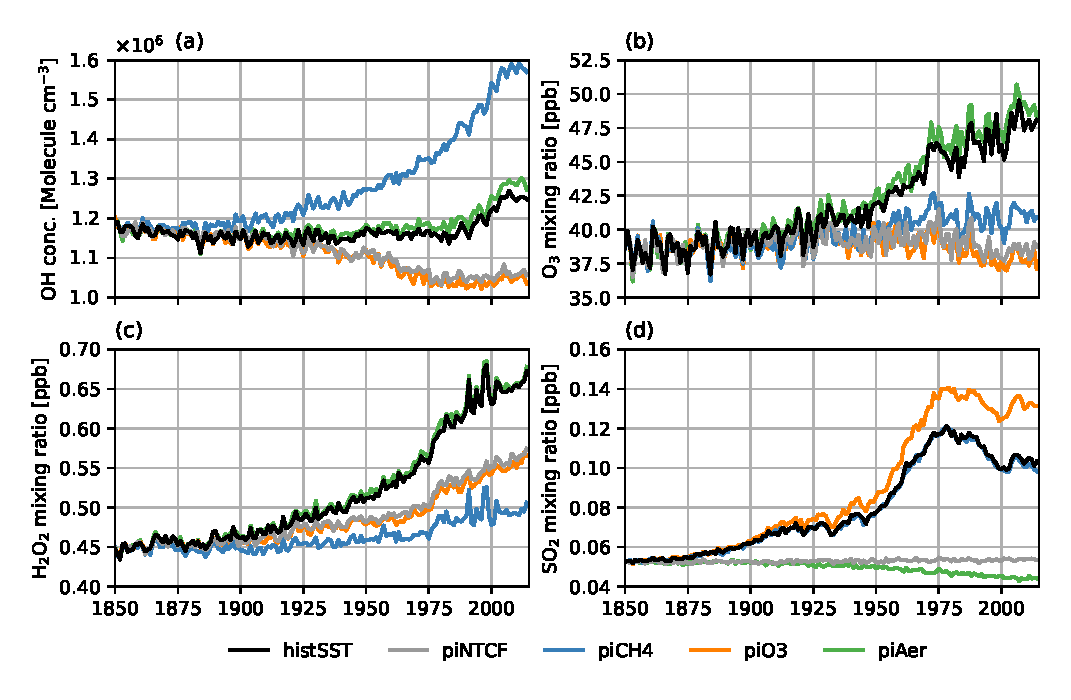
\includegraphics[width=\linewidth]{Chapter3/Figs/f02_oxidant-changes.eps}
    \caption[Global annual mean tropospheric oxidant concentrations or mixing ratios]{Global annual mean tropospheric oxidant concentrations or mixing ratios for species related to \ce{SO2} oxidation in each experiment as mentioned in Table \ref{tab:ch3:histSST-exp}.}
    \label{fig:ch3:oxidants}
\end{figure}

The historical OH concentration is stable at below \qty{1.2e6}{\per\centi\metre\cubed} until 1980, when it started to rise to \qty{1.25e6}{\per\centi\metre\cubed} by the end of 2014. In \sstpich{}, where \ce{CH4} concentration is held at the 1850 level, \ce{OH} concentrations increase above the historical trajectory because the OH sink via \ce{CH4} does not increase over time. The effect of historical increases in \ce{CH4} on OH can be seen since 1875, with the \ce{OH} concentration in 2014 increasing to 133\% that of 1850. On the other hand, in \sstpio{}, the lack of increase in \ce{O3} precursor emissions lowers OH production and hence concentration by 15\% (from \num{1.25e6} to \qty{1.05e6}{\per\centi\metre\cubed}) as shown in \sstpio{} compared to the historical trajectory, \histsst{}. This decrease is due to less OH production by the reaction of water vapour with excited oxygen atoms \ce{(O(^1D))}, which are produced by \ce{O3} photolysis ($\lambda$ < 340 nm). Aerosol precursor emissions increase \ce{SO2}, which reacts with OH. This effect is seen as an increase of \qty{0.2}{\per\centi\metre\cubed} of OH compared to the historical trajectory when comparing \histsst{} with \sstpiaer{}. In summary, the historical trend of OH is determined by \ce{CH4} and \ce{O3} precursors. The historical emission of \ce{CH4} decreases \ce{OH} concentration while \ce{O3} precursors increase the \ce{OH} concentration. These opposing forces neutralise each other, leading to a relatively stable level of OH until 1980, when the combined effects of \ce{O3} precursor and \ce{CH4} produce more OH.

\ce{O3} concentration sees a gradual increase of 26\% in the historical period from \qty{37.5}{ppb} to \qty{47.5}{ppb}. \ce{O3} precursors act mainly to increase atmospheric \ce{O3} mixing ratio. Comparing \histsst{} with \sstpio{} in Figure \ref{fig:ch3:oxidants}c, the \ce{O3} mixing ratio increases in the historical period, with \ce{O3} precursor emissions contributing to a rise of 12.5 ppb globally between 1850 and 2014. \ce{CH4} is another source of \ce{O3} as \ce{CH4} forms methyl dioxide (\ce{CH3O2}) which reacts with \ce{NO} to form formaldehyde (\ce{HCHO}). \ce{HCHO} photolysis yields \ce{CO} which is a source of tropospheric \ce{O3}. Keeping \ce{CH4} at 1850 level decreases tropospheric \ce{O3} by 7.5 ppb in 2014. 


\ce{H2O2} is not a direct climate forcing agent, but its presence indirectly affects atmospheric chemistry. The concentration of \ce{H2O2} shares a similar trend to \ce{O3} and \ce{CH4}, showing a gradual increase of \qty{0.20}{ppb} in the historical period. This correlation is due to \ce{CO}, an \ce{O3} precursor, which reacts with \ce{OH} to form \ce{HO2} and produces \ce{H2O2}. In total, \ce{O3} precursors contribute to an increase of 0.10 ppb of \ce{H2O2} in 2014. Keeping \ce{CH4} at 1850 levels, in \sstpich{}, decreases \ce{H2O2} levels as \ce{CH4} is a source of \ce{HO2} radicals, via reactions that form \ce{HCHO} and \ce{HO2} radicals (and hence \ce{H2O2}). \ce{H2O2} is 0.15 ppb higher because of \ce{CH4} increase in 2014.


Aerosol precursor emissions increase the \ce{SO2} mixing ratio in the historical period, following the historical \ce{SO2} emission trends (Figure \ref{fig:ch3:emissions}). \ce{SO2} emissions quadruple and reach their peak in 1975. This rise in emissions contributes to 0.14 ppb of \ce{SO2}, which is a 21.8\% increase from the level in 1850. \ce{O3} also directly affects \ce{SO2}. Without \ce{O3} precursor emissions, the chemical sink of \ce{SO2} is missing and results in a higher \ce{SO2} mixing ratio in \sstpio{}. The change in \ce{CH4} concentration in the historical period is shown not to affect \ce{SO2} mixing ratio. 

To summarise this section, historical \ce{O3} precursor emissions promote \ce{OH} concentration, \ce{O3} and \ce{H2O2} mixing ratio. The historical \ce{CH4} reacts away \ce{OH} but boosts \ce{O3} and \ce{H2O2} concentrations. The \ce{SO2} emissions from aerosol precursors increase the \ce{SO2} mixing ratio as its main anthropogenic source. \ce{O3} precursor emissions decrease the \ce{SO2} mixing ratio by 23.1\% (from 0.13 to 0.10 ppb) in 2014, while the historical increase in \ce{CH4} shows no effect on the \ce{SO2} mixing ratio. 


\subsection{\textsoo{} oxidation and budget changes due to historical emissions}

\subsubsection{\textsoo{} oxidation changes due to historical emissions}
\label{sec:ch3:oxidation}


In the UKESM1, \ce{SO2} reacts with \ce{OH} in the gas phase, forming sulfuric acid, which nucleates into sulfate aerosols. \ce{SO2} also reacts and with \ce{H2O2} and \ce{O3} in the aqueous phase to form sulfate aerosols. Figure \ref{fig:ch3:oxidation} shows total annual tropospheric \ce{SO2} oxidation tendencies in each pathway due to all historical emissions and due to keeping aerosol precursors, \ce{O3} precursors or \ce{CH4} at the 1850 level. 


\begin{figure}[h!]
    \centering
    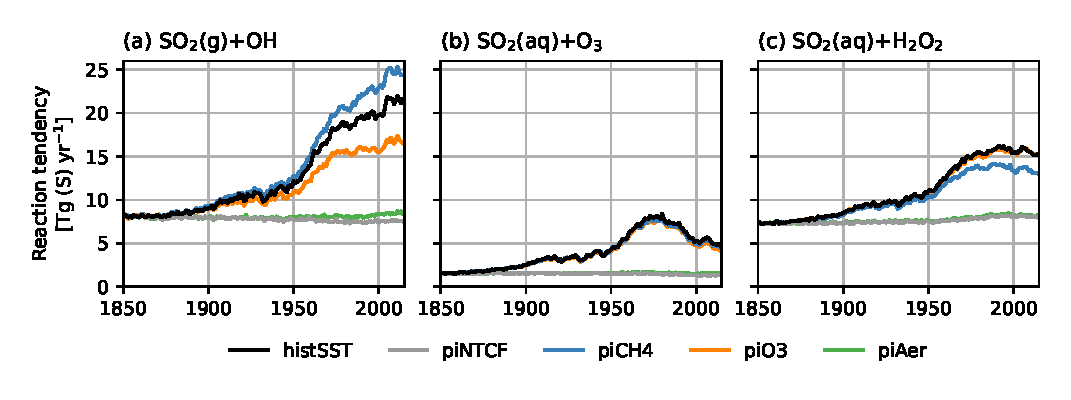
\includegraphics[width=\linewidth]{Chapter3/Figs/f03_oxidation.eps}
    \caption[Global annual \ce{SO2} oxidation tendencies]{Global annual \ce{SO2} oxidation tendencies between 1850--2014 with changes due to constraining  methane concentration (\sstpich{}), aerosol precursors (\sstpiaer{}), ozone precursors (\sstpio{}) or both emissions (\sstpintcf{}) at 1850 level.}
    \label{fig:ch3:oxidation}
\end{figure}


The \ce{SO2 + OH} trend broadly follows the \ce{SO2} emissions and the \ce{OH} concentration trends. In the historical period, \ce{SO2} oxidation by \ce{OH} increases from \qty{8.0}{Tg(S)~yr^{-1}} to \qty{22.0}{Tg(S)~yr^{-1}} between 1850--2014. The main factor for this trend is the increase in aerosol precursor emissions, as seen in the upward shift from \sstpiaer{} to \histsst{}. \ce{O3} precursor emissions and \ce{CH4} concentration were shown to increase \ce{OH} concentration in Figure \ref{fig:ch3:oxidants}. The perturbations in oxidants correspond to the changes in oxidation. The lower \ce{OH} concentration in \sstpio{} decreases \ce{SO2 + OH} reaction tendency, lowering the tendency by \qty{5.0}{Tg(S)~yr^{-1}}. With \ce{CH4} concentration constrained at the 1850 level, OH concentration in \sstpich{} rises by 30\%. This increase leads to a 19\% rise in oxidation with OH from \num{21.3} to \qty{25.0}{Tg(S)~yr^{-1}} in the near present. 


One notable result is how \ce{SO2 + O3} tendencies are not sensitive to changes in \ce{O3} mixing ratios. Figure \ref{fig:ch3:oxidants}b shows that the global \ce{O3} mixing ratio monotonically increases after 1850, but historical \ce{SO2 + O3} does not share the trend. \ce{SO2 + O3} oxidation tendency rises from \qty{2.0}{Tg(S)~yr^{-1}} to \qty{8.9}{Tg(S)~yr^{-1}} in 1975 and falls to \qty{5.0}{Tg(S)~yr^{-1}} in 2014, making this pathway the only one that does not keep increasing over the entire historical period. Despite the 25\% decrease in \ce{O3} mixing ratio in \sstpio{} and \sstpich{}, there are minimal changes to \ce{SO2 + O3} tendencies in these simulations compared to \histsst{}. The lack of change implies that globally \ce{SO2 + O3} oxidation is not sensitive to historical changes in \ce{O3} and that the background tropospheric \ce{O3} is sufficient to saturate the pathway. 


The historical \ce{H2O2} oxidation tendency measures \qty{7.5}{Tg(S)~yr^{-1}} in 1850. The tendency increases to \qty{16}{Tg(S)~yr^{-1}} and stabilises after the 1980s. A similar lack of response to oxidants in \ce{SO2 + O3} due to increases in \ce{O3} precursors is also seen in \ce{SO2} oxidation with \ce{H2O2} in \sstpio{} simulation compared to \histsst{}. The absence of anthropogenic \ce{CH4}, which is a source of \ce{H2O2} precursor, on the other hand, lowers the \ce{SO2 + H2O2} reaction tendencies by 15\% when the \ce{H2O2} mixing ratio decreases. 


Overall, the rate of \ce{SO2} oxidation with \ce{OH}, \ce{O3}, and \ce{H2O2} is controlled by \ce{SO2} abundance, as the reaction tendency tends to be constant without aerosol precursor emissions. The \ce{OH} and \ce{H2O2} pathways contribute equally to \ce{SO2} oxidation in the 1850s, but the rate of growth of \ce{SO2 + OH} oxidation is greater post-1950s, making \ce{SO2 + OH} the most important oxidising pathway. \ce{O3} is the least significant oxidant to \ce{SO2} globally, contributing to the removal of at most \qty{8.1}{Tg(S)~yr^{-1}}. The \ce{SO2 + OH} pathway is the most sensitive to oxidant changes in which the spread between \sstpio{} and \sstpich{} is approximately \qty{5.0}{Tg(S)~yr^{-1}} or 25\% of the \histsst{} oxidation rate in 2014.


To summarise the effects of historical emissions, \ce{O3} precursor emissions act to increase the gas-phase oxidation of \ce{SO2} with OH, increasing the gas-phase tendency by \qty{5}{Tg(S)~yr^{-1}} with no effects on the aqueous-phase reactions. The rise in \ce{CH4} concentration in the historical period increases the concentration of \ce{O3} and \ce{H2O2} while decreasing OH concentration with measurable impact on \ce{SO2} oxidation. In total, the historical rise in \ce{CH4} leads to a greater OH sink, decreasing \ce{SO2} oxidation with OH by \qty{4}{Tg(S)~yr^{-1}}, but adds \qty{2.5}{Tg(S)~yr^{-1}} to the \ce{SO2 + H2O2} oxidation tendency. Ultimately, \ce{CH4} decrease the total oxidation tendency globally by \qty{-1.5}{Tg(S)~yr^{-1}}, but the greater change is in shifting oxidation from gas- to aqueous-phase.


\subsubsection{\textsoo{} and \textsoooo{} burdens, losses, lifetimes, and budgets and changes due to historical emissions}


An atmospheric chemical budget is a way to account for the global source, sink, and atmospheric burden of a trace gas. The lifetime of a trace gas describes how long it stays in the atmosphere and is defined as the average time that a molecule of that species remains in a reservoir before removal. When the reservoir is the whole atmosphere, and the trace gas is in a steady state, the burden is considered constant, and the tropospheric lifetime of a compound is estimated by dividing the total tropospheric burden by total loss. 

Oxidants affect the \ce{SO2} budget in various ways. So far, this chapter has quantified the source for \ce{SO2} and \ce{SO4} through \ce{SO2} oxidation. In this section, \ce{SO2} loss terms include chemical losses via oxidation with \ce{OH}, \ce{O3}, and \ce{H2O2}, and wet and dry deposition are analysed. 


\ce{SO2} reacts with \ce{OH}, \ce{H2O2} and \ce{O3} to form sulfate so the budget of \ce{SO2} and \ce{SO4} are connected via these oxidation processes. Figure \ref{fig:ch3:s-budget} shows global and annual burdens, loss processes, and lifetimes of \ce{SO2} and \ce{SO4} in the troposphere. Table \ref{tab:ch3:budget-pothole}, \ref{tab:ch3:budget-near-present} and figure \ref{fig:ch3:so2-losses-bar} quantify the budget for 1960--1989 and 2000--2014 inclusive. These two periods are chosen for their high \ce{SO2} emissions. Both \ce{SO2} and \ce{SO4} are assumed to be in steady-state, and the lifetimes are calculated from the total burden divided by the total losses.


\begin{figure}[h!]
    \centering
    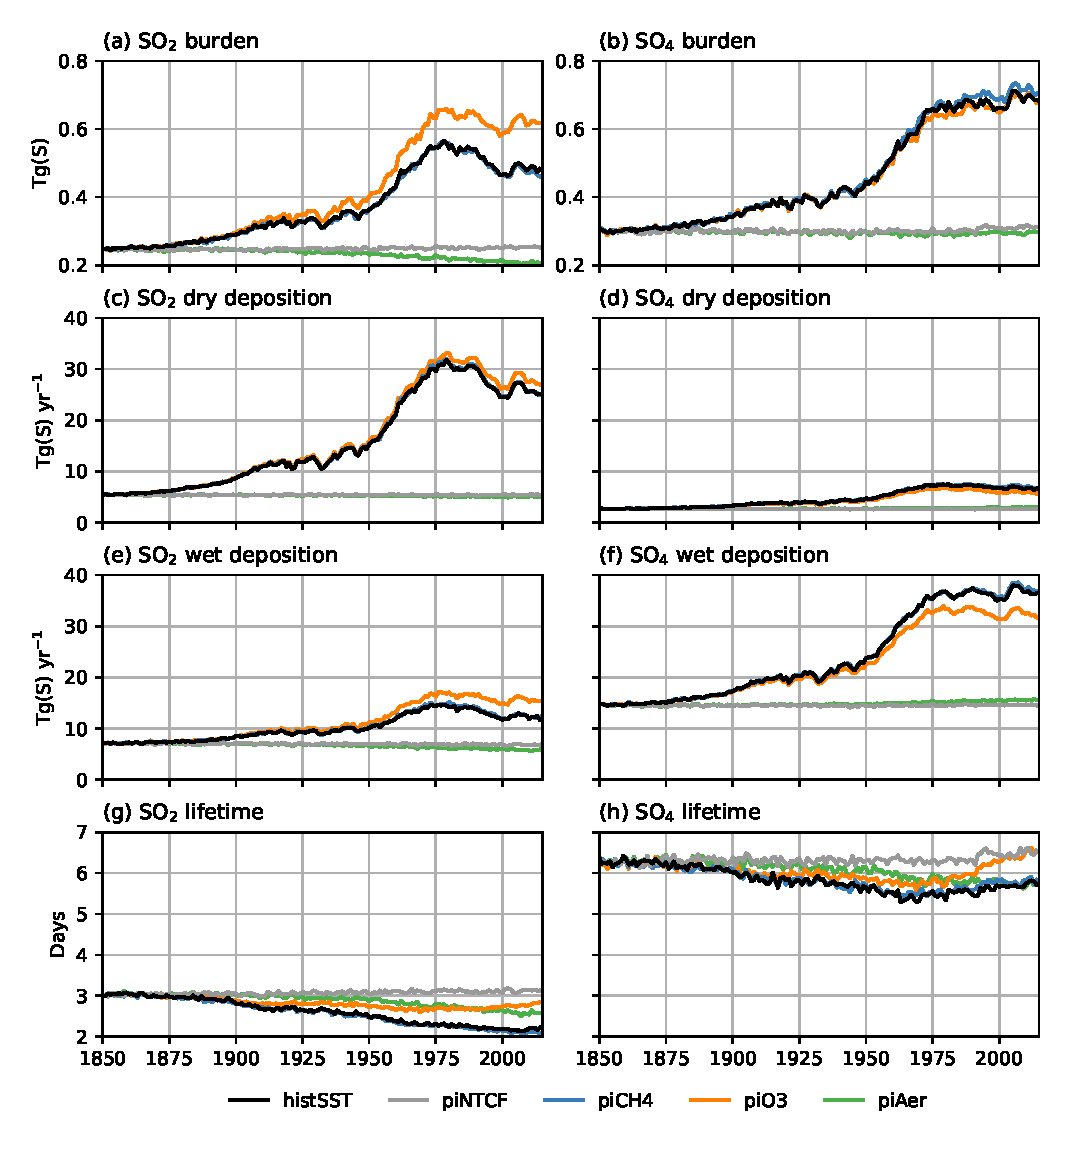
\includegraphics[width=\linewidth]{Chapter3/Figs/f04_s-budget.eps}
    \caption[Tropospheric sulfur budget terms including burdens, depositions and lifetimes]{Tropospheric \ce{SO2} and \ce{SO4} budget, including (a-b) burdens, (c-d) dry depositions, (e-f) wet depositions, and (g-h) lifetimes. The plots show budget terms between 1850 and 2014 with changes due to constraining  methane concentration (\sstpich{}), aerosol precursors (\sstpiaer{}), ozone precursors (\sstpio{}) or both emissions (\sstpintcf{}) at the 1850 level.}
    \label{fig:ch3:s-budget}
\end{figure}


\begin{figure}[h!]
    \centering
    \includegraphics{Chapter3/Figs/so2_losses_bar.png}
    \caption[Global annual \ce{SO2} oxidation tendencies in 1960--1989 and 2000-2014]{Global annual \ce{SO2} oxidation tendencies in 1960--1989 and 2000-2014 with changes due to constraining \ce{CH4} concentration (\sstpich{}), aerosol precursors (\sstpiaer{}), ozone precursors (\sstpio{}) or both emissions (\sstpintcf{}) at 1850 level.}
    \label{fig:ch3:so2-losses-bar}
\end{figure}

\begin{table}[h!]
   \caption[Summary of tropospheric sulfur budget between 1960--1989]{Summary of tropospheric sulfur budget from relevant UKESM1 AerChemMIP simulations  covering the period 1960--1989 inclusive. Units for emission and loss tendencies are in \unit{Tg(S)~yr^{-1}}. Burdens are in \unit{Tg(S)}, and lifetimes are in days. Numbers in parentheses are the fractions of production or loss.}
   \label{tab:ch3:budget-pothole}
    \centering
\begin{tabular}{l p{14mm} p{14mm} p{14mm} p{14mm} p{14mm}}

\toprule
& \histsst{} & \sstpio{} & \sstpich{} & \sstpiaer{} & \sstpintcf{} \\

\midrule
\ce{SO2} \\
\midrule

Primary emission & 72.72 & 72.72 & 72.72 & 15.23 & 15.23 \\
\ce{SO2 (g) + OH} & 17.71 \textit{(21.5)} & 14.88 \textit{(18.0)} & 19.51 \textit{(23.5)} & 8.05 \textit{(27.8)} & 7.53 \textit{(25.9)} \\
\ce{SO2 (aq) + O3} & 7.47 \textit{(9.1)} & 7.08 \textit{(8.6)} & 7.22 \textit{(8.7)} & 1.61 \textit{(5.5)} & 1.46 \textit{(5.0)} \\
\ce{SO2 (aq) + H2O2} & 14.77 \textit{(17.9)} & 14.54 \textit{(17.6)} & 13.32 \textit{(16.0)} & 7.98 \textit{(27.5)} & 7.82 \textit{(26.9)} \\
Total oxidation & 39.95 \textit{(48.5)} & 36.50 \textit{(44.2)} & 40.05 \textit{(48.2)} & 17.63 \textit{(60.9)} & 16.80 \textit{(57.8)} \\
Dry deposition & 28.63 \textit{(34.7)} & 30.03 \textit{(36.4)} & 28.88 \textit{(34.8)} & 5.11 \textit{(17.6)} & 5.37 \textit{(18.5)} \\
Wet deposition & 13.85 \textit{(16.8)} & 16.04 \textit{(19.4)} & 14.14 \textit{(17.0)} & 6.23 \textit{(21.5)} & 6.88 \textit{(23.7)} \\
Total deposition & 42.48 \textit{(51.5)} & 46.07 \textit{(55.8)} & 43.02 \textit{(51.8)} & 11.33 \textit{(39.1)} & 12.26 \textit{(42.2)} \\
Total loss & 82.42 & 82.57 & 83.07 & 28.97 & 29.06 \\
Burden & 0.53 & 0.61 & 0.52 & 0.22 & 0.25 \\
Lifetime & 2.29 & 2.67 & 2.27 & 2.76 & 3.11  \\

\midrule
\ce{SO4}  \\
\midrule

Primary emission & 1.87 \textit{(4.5)} & 1.87 \textit{(4.9)} & 1.87 \textit{(4.5)} & 0.39 \textit{(2.2)} & 0.39 \textit{(2.3)} \\
Secondary emission & 39.95 \textit{(95.5)} & 36.50 \textit{(95.1)} & 40.05 \textit{(95.5)} & 17.63 \textit{(97.8)} & 16.80 \textit{(97.7)} \\
Total emission & 41.81 & 38.37 & 41.91 & 18.02 & 17.20 \\
Dry deposition & 6.95 \textit{(16.7)} & 6.31 \textit{(16.5)} & 7.02 \textit{(16.8)} & 2.80 \textit{(15.6)} & 2.61 \textit{(15.3)} \\
Wet deposition & 34.65 \textit{(83.3)} & 31.86 \textit{(83.5)} & 34.67 \textit{(83.2)} & 15.15 \textit{(84.4)} & 14.51 \textit{(84.7)} \\
Total loss & 41.6 & 38.16 & 41.69 & 17.95 & 17.13 \\
Burden & 0.63 & 0.62 & 0.64 & 0.29 & 0.30 \\
Lifetime & 5.46 & 5.81 & 5.53 & 5.84 & 6.30 \\
\midrule
Total \ce{SO2} and \ce{SO4} lifetime & 4.95 & 5.25 & 4.95 & 6.31 & 6.75 \\
\bottomrule

\end{tabular}
\end{table}


\begin{table}[h!]
   \caption[Summary of tropospheric sulfur budget between 2000--2014]{Summary of tropospheric sulfur budget from relevant UKESM1 AerChemMIP simulations  covering the period 2000--2014 inclusive. Units for emission and loss tendencies are in \unit{Tg(S)~yr^{-1}}. Burdens are in \unit{Tg(S)}, and lifetimes are in days. Numbers in parentheses are the fractions of production or loss.}
   \label{tab:ch3:budget-near-present}
    \centering
\begin{tabular}{l p{14mm} p{14mm} p{14mm} p{14mm} p{14mm}}

\toprule
& \histsst{} & \sstpio{} & \sstpich{} & \sstpiaer{} & \sstpintcf{} \\

\midrule
\ce{SO2} \\
\midrule

Primary emission & 69.68 & 69.68 & 69.68 & 15.23 & 15.23 \\
\ce{SO2 (g) + OH} & 21.14 \textit{(26.4)} & 16.61 \textit{(20.7)} & 24.39 \textit{(30.1)} & 8.44 \textit{(29.1)} & 7.58 \textit{(26.0)} \\
\ce{SO2 (aq) + O3} & 5.17 \textit{(6.5)} & 4.67 \textit{(5.8)} & 4.96 \textit{(6.1)} & 1.53 \textit{(5.3)} & 1.29 \textit{(4.4)} \\
\ce{SO2 (aq) + H2O2} & 15.54 \textit{(19.4)} & 15.54 \textit{(19.4)} & 13.40 \textit{(16.6)} & 8.20 \textit{(28.3)} & 8.07 \textit{(27.7)} \\
Total oxidation & 41.86 \textit{(52.3)} & 36.81 \textit{(45.9)} & 42.75 \textit{(52.8)} & 18.18 \textit{(62.7)} & 16.94 \textit{(58.1)} \\
Dry deposition & 25.85 \textit{(32.3)} & 27.77 \textit{(34.7)} & 25.86 \textit{(31.9)} & 5.02 \textit{(17.3)} & 5.42 \textit{(18.6)} \\
Wet deposition & 12.29 \textit{(15.4)} & 15.55 \textit{(19.4)} & 12.36 \textit{(15.3)} & 5.80 \textit{(20.0)} & 6.79 \textit{(23.3)} \\
Total deposition & 38.15 \textit{(47.7)} & 43.32 \textit{(54.1)} & 38.21 \textit{(47.2)} & 10.83 \textit{(37.3)} & 12.21 \textit{(41.9)} \\
Total loss & 80.00 & 80.13 & 80.96 & 29.00 & 29.15 \\
Burden & 0.48 & 0.62 & 0.47 & 0.21 & 0.25 \\
Lifetime & 2.17 & 2.77 & 2.11 & 2.58 & 3.13 \\

\midrule
\ce{SO4}  \\
\midrule

Primary emission & 1.79 \textit{(4.1)} & 1.79 \textit{(4.6)} & 1.79 \textit{(4.0)} & 0.39 \textit{(2.1)} & 0.39 \textit{(2.3)} \\
Secondary emission & 41.86 \textit{(95.9)} & 36.81 \textit{(95.4)} & 42.75 \textit{(96.0)} & 18.18 \textit{(97.9)} & 16.94 \textit{(97.7)} \\
Total emission & 43.65 & 38.60 & 44.53 & 18.57 & 17.33 \\
Dry deposition & 6.72 \textit{(15.5)} & 5.90 \textit{(15.4)} & 7.00 \textit{(15.8)} & 2.92 \textit{(15.8)} & 2.66 \textit{(15.4)} \\
Wet deposition & 36.67 \textit{(84.5)} & 32.45 \textit{(84.6)} & 37.26 \textit{(84.2)} & 15.57 \textit{(84.2)} & 14.60 \textit{(84.6)} \\
Total loss & 43.39 & 38.35 & 44.26 & 18.49 & 17.26 \\
Burden & 0.69 & 0.69 & 0.71 & 0.29 & 0.31 \\
Lifetime & 5.71 & 6.44 & 5.79 & 5.74 & 6.48 \\
\midrule
Sulfur lifetime & 5.17 & 5.75 & 5.18 & 6.17 & 6.89 \\
\bottomrule

\end{tabular}
\end{table}


Figure \ref{fig:ch3:s-budget} shows that \ce{SO2} burden trend follows that of \ce{SO2} emissions in Figure \ref{fig:ch3:emissions} and rises over time, with the burden doubling from \num{0.25} to \qty{0.48}{Tg(S)} between 1850 and 2014. The lack of historical \ce{O3} precursor emissions in \sstpio{} increases \ce{SO2} burden, starting in 1900 and led to additional \qty{0.14}{Tg(S)} burden in 2014 compared to \histsst{}. Similar responses to \ce{SO2} burden is also observed in low \ce{SO2} emission scenarios when comparing \sstpiaer{} and \sstpintcf{}, with \sstpintcf{} showing additional \qty{0.04}{Tg(S)} of \ce{SO2} burden. This is attributable to the decrease in oxidative losses of \ce{SO2} with \ce{OH}. It could be seen that historical changes in \ce{CH4} do not modify the \ce{SO2} burden.

The combination of wet and dry deposition is responsible for about half of \ce{SO2} loss at the start of 1850 in the historical simulation, \histsst{}. In 1850, wet and dry deposition tendencies are comparable, and account for \num[]{6.88} and \qty{5.37}{Tg(S)~yr^{-1}}, respectively, which is 57.8\% of total \ce{SO2} losses. The deposition trends follow \ce{SO2} emissions, with dry deposition increasing faster than wet deposition, with dry deposition increasing fivefold while wet deposition only doubles in 2014. Comparing \histsst{} and \sstpiaer{}, quadrupling historical \ce{SO2} emissions between 1850 and 2014 shifts the percentage of \ce{SO2} loss by deposition from 37.3\% to 47.7\%. One explanation is that, unlike volcanic \ce{SO2}, which is emitted at altitudes above the surface, anthropogenic \ce{SO2} is emitted at the model surface level, where dry deposition is efficient. This means in \histsst{} a larger percentage of \ce{SO2} is emitted close to the surface compared to \sstpiaer{}. The other reason could be that, as a result of increased \ce{SO2} emissions, the atmosphere does not have the capacity to oxidise all the additional \ce{SO2}, so a greater proportion of \ce{SO2} is being removed by deposition. When comparing \histsst{} and \sstpio{}, it could be seen again that increasing the historical \ce{O3} precursor emissions affects the \ce{SO2} budget. In 2014, historical \ce{O3} precursor emissions lower \ce{SO2} wet and dry deposition by \qty{5.17}{Tg(S)~yr^{-1}}. Despite this change, the total loss of \ce{SO2} in \sstpio{} only differs from that of \histsst{} by \qty{0.13}{Tg(S)~yr^{-1}}. This suggests that oxidation outcompetes oxidation in removing \ce{SO2} from the atmosphere when oxidant levels increase and the loss is away from the surface, where dry deposition dominates, resulting in approximately unchanged total loss. The historical increase in \ce{CH4} does not significantly affect wet and dry deposition of \ce{SO2} throughout the simulation period.


Atmospheric burden, loss and lifetime are correlated when the chemical species is in a steady state. The atmospheric lifetime can be calculated by dividing the burden by the total loss, and the tropospheric lifetime of \ce{SO2} is 3.1 days in the 1850s. The lifetime decreases over the historical period to 2.17 days in 2014 for the historical simulation. Similar downward trends are observed in all simulations, at various degrees of reduction, except \sstpintcf{}. The decrease is partially attributed to \ce{O3} precursors and aerosol precursor emissions. When the aerosol and \ce{O3} precursors emission are kept at the 1850 level in \sstpintcf{}, the atmosphere's oxidative capacity remained constant, and \ce{SO2} lifetime is unchanged throughout the period. This could imply that \ce{SO2} oxidation is not sensitive to historical sea surface temperature changes, but the availability of oxidants drives the change in \ce{SO2} budget. \ce{CH4}, which is a sink for OH and a source for \ce{O3} and \ce{H2O2}, shifts the oxidation towards more aqueous-phase oxidation, which is compensated by lower \ce{SO2 + OH}. Since the total \ce{SO2} loss remains unchanged in \sstpich{} compared to \histsst{}, it could be said that the historical change in \ce{CH4} does not impact the lifetime of \ce{SO2}.


In UKESM1, sulfate aerosols are emitted as primary emissions or formed in the atmosphere through oxidation, with the most sulfate aerosols being produced via oxidation. For example, between 1960 and 1989, \num{1.87} and \qty{39.95}{Tg(S)~yr{-1}} of sulfate production in the UKESM1 historical simulation are attributed to secondary production via primary emission and oxidation, respectively (Table \ref{tab:ch3:budget-pothole}). The sulfate burden increases from \num{0.30} to \qty{0.69}{Tg(S)} between 1850 and 2014 in the historical simulation. The increase directly correlates to \ce{SO2} emissions and the subsequent \ce{SO2} oxidation. Historical changes in \ce{O3} precursor and \ce{CH4} minimally affect sulfate aerosol burden. 


Wet deposition is an efficient process for removing sulfate aerosols in the atmosphere because the aerosols are soluble. The two methods of removal increase over time to reflect more production in the historical simulations, with the ratio between the two removal processes being constant over time. Wet deposition removes 83--85\% of sulfate aerosols compared to dry deposition across time and in all simulations. \ce{O3} precursors affect the total sulfate removal processes tendency in the historical period because less sulfate is produced from oxidation, while historical \ce{CH4} emissions have minimal effects on sulfate removal.

The lifetime of sulfate aerosols is 6.3 days, decreasing to 5.41 days from 1960 to 1989, and rebounds slightly to 5.71 days at the end of the historical simulations. By comparing \sstpintcf{}{} with \sstpiaer{} and \sstpio{}, it could be seen that the increase in \ce{SO2} emissions and \ce{O3} precursors affects sulfate lifetime in different ways. The increase in aerosol precursor emissions reduces the sulfate lifetime by 0.49 days (6.30 minus 5.81 days) in 1960--1898 but only 0.04 days in 2000--2014. The main difference in \ce{SO2} emission between the two periods is in their emission location, i.e. in 1960--1989 the majority of \ce{SO2} is emitted in Europe and Northeast America, while, in the latter period, emissions from Europe have drastically decreased and emissions from East and South Asia rose. Chapter \ref{ch5:title} further explores the impact of emission location on sulfate aerosol formation. Historical changes in \ce{O3} precursor alone gradually shorten sulfate aerosol lifetime, from 6.30 days to 5.84 days and 5.74 days, in 1850, 1960--1989, and 2000--2010, respectively, as seen in Table \ref{tab:ch3:budget-pothole}--\ref{tab:ch3:budget-near-present} for \sstpiaer{}.


To summarise, historical \ce{O3} precursor emissions act to increase oxidation. Consider the counterfactual historical simulation \sstpio{} compared to \histsst{}, the higher levels of \ce{O3} precursors in \sstpio{} result in increment of \ce{SO2 + OH} oxidation by \qty{4.53}{Tg(S)~yr^{-1}}, while dry deposition decreases by \qty{-1.92}{Tg(S)~yr^{-1}} in 2000--2014. With the greater total loss, \ce{SO2} burden decreases, shortening \ce{SO2} lifetime by 0.6 days (14.4 hours). The increased oxidation affects the sulfate budget. Sulfate wet and dry deposition increases to reflect more secondary sulfate production. Consequently, the global sulfate burden remains the same as \histsst{}. Since the sulfate burden is unchanged but loss decreases, the sulfate lifetime is 0.73 days shorter due to co-emission of \ce{SO2} and \ce{O3} precursors. Therefore, it can be said that \ce{O3} precursor emissions increase \ce{SO2 + OH} oxidation and shorten \ce{SO2} and sulfate lifetime as \ce{O3} precursors increase the atmospheric oxidative power.

\ce{O3} precursor emission's impacts on sulfur budgets can also be seen by comparing \sstpiaer{} and \sstpintcf{}. In both simulations, \ce{SO2} emissions are kept at the 1850 level throughout the historical period. In \sstpintcf{}, \ce{O3} precursor emissions are also kept at the 1850 level. \ce{SO2 + OH} oxidation tendency increases over the historical period in \sstpiaer{} as shown in Figure \ref{fig:ch3:s-budget}. The historical \ce{SO2} burden and lifetime slightly decrease over time as a response. Again, \ce{O3} precursors are shown to increase \ce{SO2 + OH} oxidation.


Effects of co-emissions of \ce{O3} precursors with \ce{SO2} can be quantified by comparing two pairs of simulations:\histsst{}/\sstpio{} and \sstpiaer{}/\sstpintcf{}. Increased \ce{O3} precursors emissions in the atmosphere with high \ce{SO2} results in a 5.7\% promotion in \ce{SO2 + OH} oxidation (\histsst{}/\sstpio{}). Only a 3.1\% increase is seen in the low \ce{SO2} atmosphere in the 2000--2014 period (\sstpiaer{}/\sstpintcf{}). This further indicates the role of \ce{O3} in the \ce{SO2} budget via oxidation with \ce{OH}. Therefore, it can be said that co-emissions of \ce{O3} precursors with \ce{SO2} result in a larger increase in \ce{SO2 + OH} oxidation. 


Increases in \ce{CH4} concentrations affect oxidants that \ce{SO2} reacts with. Comparing \histsst{} and \sstpich{}, \ce{SO2 + OH} decreases by \qty{-3.25}{Tg(S)~yr^{-1}} from 24.39 to \qty{21.14}{Tg(S)~yr^{-1}}. However, The total oxidation decreases only by \qty{-0.89}{Tg(S)~yr^{-1}} as there is an opposing increase of \num{0.21} and \qty{2.14}{Tg(S)~yr^{-1}} in \ce{O3} and \ce{H2O2} oxidation with \ce{SO2}, respectively. \ce{SO2} burden stays roughly the same when \ce{CH4} concentration is kept at 1850 level in \sstpich{}, despite the huge differences in \ce{CH4} and as a result OH (see Figure \ref{fig:ch3:emissions}). In summary, the increase in \ce{CH4} significantly reduces gas-phase oxidation and increases aqueous-phase oxidation but leaves other sulfur budget terms unchanged.



\citet{karsetStrongImpactsAerosol2018} quantified the effect of oxidants on \ce{SO2} lifetime. By replacing oxidants (\ce{NO3}, \ce{O3}, \ce{OH} and \ce{HO2}) from present-day to pre-industrial, the lifetime of pre-industrial \ce{SO2} increased from 29 hours (1.21 days) to 34 hours (1.42 days), which was an increase by 17\%. This conclusion is similar to the work in this thesis, which shows a 28\% increase in \ce{SO2} lifetime from 2.17 days to 2.77 days due to constraining \ce{O3} precursor emissions to 1850, a similar pre-industrial condition.  



\subsection{Aerosol properties changes due to SLCFs}

\ce{SO2} oxidation determines aerosol microscopic and macroscopic properties. In UKESM1, \ce{SO2} oxidises with OH and produces sulfuric acid, which nucleates into new aerosol particles \citep{mannDescriptionEvaluationGLOMAPmode2010}. In contrast, aqueous-phase oxidation adds mass to existing accumulation- and coarse-mode aerosol without creating new particles. In the previous section, changes over the historical period have been shown to perturb the proportion of \ce{SO2} being oxidised in the gas or aqueous phase. The described oxidation changes may impact aerosol properties, especially aerosol size distribution. Once formed, aerosols undergo various processes that further modify their bulk properties. Aerosols may grow by coagulation or be removed by deposition. These aerosol processes are simulated in UKESM1 using the GLOMAP-mode aerosol scheme. This section investigates historical aerosol properties and the changes to aerosol properties from SLCF emissions.  

Aerosol optical depth (AOD) is a dimensionless number that measures the amount of incoming solar radiation that atmospheric particles prevent from reaching the surface. The amount of aerosol in the atmosphere is linked to \ce{SO2} oxidation tendency as oxidation produces \ce{SO4} aerosols. Figure \ref{fig:ch3:AOD} shows annual global mean AOD from fixed-SST simulations. It illustrates that historical emissions increase AOD by 50\% in 2014 and are the main contributor to global AOD. AOD in the \sstpio{} simulation is 0.05 lower than \histsst{}, suggesting that \ce{O3} contributes to aerosol loading. Global AOD is unchanged under lower \ce{CH4} condition in \sstpich{}.


\begin{figure}[h!]
    \centering
    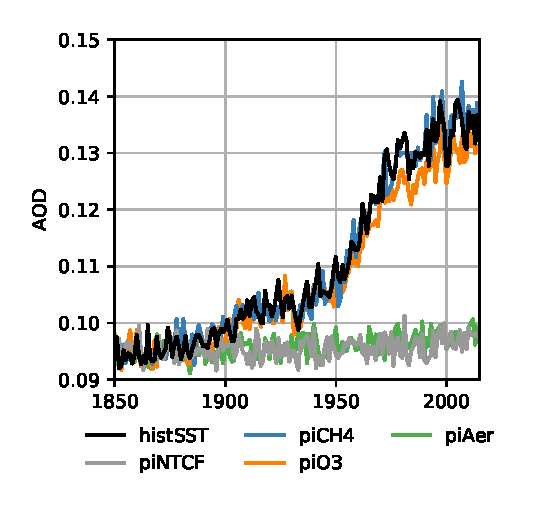
\includegraphics{Chapter3/Figs/f05_aod-trend.eps}
    \caption[Global annual mean AOD between 1850-2014 with changes due to SLCFs]{Global annual mean AOD between 1850-2014 (\histsst{}) with changes due to constraining the following SLCFs at the 1850 level: methane concentration (\sstpich{}), aerosol precursors (\sstpiaer{}), ozone precursors (\sstpio{}) or both aerosol precursor and ozone precursor emissions (\sstpintcf{}).}
    \label{fig:ch3:AOD}
\end{figure}


In addition to global trends, the spatial pattern of AOD gives insight into the distribution of AOD to locate its potential climate impact. Figure \ref{fig:ch3:AOD-map} shows the distribution of AOD and changes due to historical \ce{O3} precursor emissions and \ce{CH4} between 1980 and 1989, when emissions are most significant from North America and Europe. Unhatched areas in subfigure b--d denote statistically significant differences between \histsst{} and each counterfactual simulation ($p \leq 0.05$). Areas with elevated AOD include Sub-Saharan Africa, Central America, Northeast America, Central Europe, and Eastern Asia. Apart from Sub-Saharan Africa and Central America, aerosol precursor emissions are responsible for increases in AOD in the 1980s. \ce{O3} precursors are responsible for 20\% of AOD in high-emission areas (0.08 out of 0.4 over the European region, for example). \ce{CH4} has an insignificant effect on AOD. This is due to the nullifying nature of the change: increase of \ce{SO2 + OH} oxidation and the decrease in \ce{SO2 + H2O2}, which results in approximately net zero change in total oxidation tendency compared to \histsst{}. Although reaction tendency has shifted due to \ce{CH4}, some aerosol diagnostics, such as AOD, may remain unchanged. 


\begin{figure}[h!]
    \centering
    \includegraphics[width=\linewidth]{Chapter3/Figs/f06_aod-map.png}
    \caption[Mean AOD at 550 nm from 1980-1989 and changes to AOD due to SLCFs]{(a) Decadal mean AOD at 550 nm from 1980-1989. (b-d) Difference of AOD at 550 nm from 1980-1989 between \histsst{} and \sstpiaer{}, \sstpio{}, and \sstpich{}, respectively. Hatched areas denote areas where the difference is not statistically significant ($p \leq 0.05$).}
    \label{fig:ch3:AOD-map}
\end{figure}


One significant improvement in the GLOMAP-mode aerosol scheme over its predecessor, the CLASSIC scheme, is its ability to independently simulate aerosol size and number for aerosol species and distributions. Aerosols are simulated in four modes according to their diameter: nucleation, Aitken, accumulation and coarse. Figure \ref{fig:ch3:aerosol-size-dist-time} shows, in the top row, the aerosol size distribution for aerosol with a diameter between \qty{1}{\nano\metre} and \qty{10}{\micro\metre} at 1 km above the surface for the period 2010--2014. Aerosol at 1 km altitude is chosen for its relevance to cloud formation. Along with historical aerosol size distribution, top panels (a--c) show percentage changes in aerosol size distributions due to aerosol precursor emissions, \ce{O3} precursor emissions and \ce{CH4} concentration calculated by subtracting \histsst{} with \sstpiaer{}, \sstpio{} and \sstpich{}, respectively. The bottom panels (d--f) show the progression of change in aerosol size over time. In the bottom panels, each horizontal stripe denotes the percentage difference of global decadal mean aerosol size distribution at 1 km between \histsst{} and the perturbed simulations. For example, the percentage differences for 2010--2014 in figures (a--c) are plotted as the topmost colour bar in figures (d--f). Vertical dashed lines in all panels mark the location of aerosol diameter equal to \qty{50}{\nano\metre}. The subset of aerosol with a diameter above \qty{50}{\nano\metre} is called N50 and is an important cloud condensation nuclei. This will be relevant in the next section.


\begin{figure}[ht]
    \centering
    \includegraphics[width=0.8\linewidth]{Chapter3/Figs/f08_aerosol-size-dist-over-time.png}
    \caption[Aerosol size distribution for 2010-2014 at 1 km]{(top) Historical total aerosol size distribution at 1 km for 2010-2014 with percentage difference on the secondary axis. (bottom) The progression of percentage change of aerosol size distribution due to (d) aerosol precursors, (e) \ce{O3} precursors, and (f) \ce{CH4}. The vertical dashed line denotes the 50 nm diameter (25 nm radius) above which aerosol affects cloud nucleation.}
    \label{fig:ch3:aerosol-size-dist-time}
\end{figure}


As shown by figure \ref{fig:ch3:aerosol-size-dist-time}d, historical aerosol precursor emissions increase aerosol concentrations in all sizes over time, with the greatest for nucleation mode aerosols between 1960 and 1989, when aerosol with diameters smaller than 50 nm increased by more than 40\%. The increase in aerosol with a diameter below 50 nm stopped and decreased after 1990. Aerosol with a diameter above 50 nm, on the other hand, increased monotonically to 30-35\% in 2014. These larger aerosols are more likely to affect the concentration of cloud condensation nuclei (CCN) \citep{seinfeldAtmosphericChemistryPhysics2016}. 

Figure \ref{fig:ch3:aerosol-size-dist-time}e shows the percentage increase in aerosol abundance due to historical \ce{O3} precursors. The aerosols with a diameter below 50 nm increase until reaching a maximum in the 1970s, a trend similar to changes from aerosol precursor emissions. While \ce{O3} precursors substantially increase the number of aerosols with a diameter smaller than 50 nm, they minimally increase the number with diameters above 50 nm, increasing the number by approximately 4\%. Consistent with Section \ref{sec:ch3:oxidation}, it could be said that the \ce{O3} precursor's effect is to increase the \ce{SO2 + OH} reaction tendency, forming sulfuric acid, which nucleates into new sulfate aerosol particles. 

Consider the effects of historical \ce{CH4} emissions, figure \ref{fig:ch3:aerosol-size-dist-time}f shows a complex picture of decreasing abundance of aerosols with a diameter below 5,000 nm but increasing the number of with a diameter above 1000 nm by 8\% after the 1970s. However, the number concentration of aerosols with this size is only 1--2 particles per \unit{\centi\metre\cubed}, rendering the 8\% change negligible. More importantly, an increase in \ce{CH4} concentration decreases the aerosol number with a diameter up to 300 nm by 15\%. This is more significant as the number concentration of aerosol with this size is one order of magnitude in the range of 10--100, as shown in subfigure (c). That is, increases in \ce{CH4} inhibit new aerosol formation by decreasing \ce{SO2 + OH} reaction tendency and increasing \ce{SO2 + H2O2} tendency, which does not result in new aerosol particles, but only increases the size of existing sulfate aerosol particles.

Aerosol precursor emissions include many aerosol types, but studies have shown that \ce{SO2} is the primary contributor to the historical increase in AOD. According to a multi-model study by \citet{kalisorasDecomposingEffectiveRadiative2024}, the total aerosol precursor emissions in CMIP6 simulations could be decomposed into impacts by \ce{SO2}, which is a precursor for sulfate aerosols, organic carbon precursors, and black carbons. Results for UKESM1 in this study showed that optical depth from \ce{SO2} contributed 79.0\% of total aerosol AOD (0.0260 from 0.0329), as shown in Table S1 of \citet{kalisorasDecomposingEffectiveRadiative2024}.

% add discussions on the results by O'Connor
The results for aerosol size distribution due to historical \ce{CH4} concentration discussed in this chapter agree with the work of \citet{oconnorApportionmentPreIndustrial2022}, which reported a change in aerosol size distribution due to \ce{CH4}. They found that an increase in \ce{CH4} concentration in the present day led to a significant reduction in aerosol number concentration in the Aitken and accumulation modes. The decrease in N50 occurred across all latitudes and through the depths of the atmosphere. As \citet{oconnorApportionmentPreIndustrial2022} used time-slice simulations in their work, this chapter adds to their finding that the reduction in N50 occurs as early as the 1920s and increases in magnitude over time, to a maximum relative difference of 15\% in 2010. 

In summary, this section has quantified the impact of oxidant perturbation due to historical \ce{O3} precursors and \ce{CH4}. \ce{O3} precursors act to increase AOD as it contribute to \ce{SO2 + OH} oxidation. The aerosols with diameters less than \qty{50}{nm} see the largest increase. \ce{CH4} reduces number of aerosols with diameter below \qty{300}{nm} but does not significantly modify AOD.


\subsection{Cloud properties changes due to SLCFs}

Aerosols act as germs for cloud formation and modify cloud properties. Aerosol particles large enough to activate water vapour condensation are called cloud condensation nuclei  \citep[CCN; ][]{aitkenDustFogsClouds1881,kohlerNucleusGrowthHygroscopic1936, bellouinBoundingGlobalAerosol2020}. This way, more numerous CCNs lead to increasing cloud droplet number concentration (CDNC) and imply a decrease in cloud droplet effective radius \citep[\Reff{}; ][]{bellouinBoundingGlobalAerosol2020}. 


Cloud properties are susceptible to feedback from warming tropospheric temperatures, which may be induced by \ce{CH4} or \ce{O3} or cooling due to aerosols. Still, the experiment design of fixed-SST simulations in AerChemMIP mitigates this issue. Cloud feedback refers to the changes in cloud properties and behaviours in response to a warming climate, which in turn affect the Earth's radiative balance and amplify or dampen global warming \citep{wangCompensationCloudFeedback2021, grosvenorChangeAerosoldrivenCloudfeedbackdriven2023}. Fixed-SST simulations used in this chapter are atmosphere-only simulations with fixed sea-surface temperatures. This simulation design rules out the impact of temperature due to cloud feedback and allows for investigation of the effects of changes in chemistry on clouds when comparing between \histsst{} and the perturbed runs during the same period. 

Although UKESM1 interactively simulates CCN using aerosol size distribution, composition, and meteorological conditions, the simulated CCN number concentrations were not archived in AerChemMIP simulations by UKESM1 used in this thesis. Therefore, aerosols with a diameter above \qty{50}{nm} (N50) are assumed to act as CCNs in which their concentration modifies cloud properties. Figure \ref{fig:ch3:cloud} shows the global decadal mean N50 concentration and cloud properties, including CDNC, \Reff{} and cloud fraction at 1 km, assumed to be in the low-level clouds. The historical simulation shows a 50\% increase in N50 from \qty{390.7}{\per\centi\metre\cubed} to \qty{602.1}{\per\centi\metre\cubed} by the end of 1990, when the increment stopped and dropped slightly to \qty{572.7}{\per\centi\metre\cubed}. Aerosol precursor emissions are responsible for the significant increase in N50 when contrasting \histsst{} and \sstpiaer{}. Historical \ce{O3} precursor emissions contribute to one third of N50 in the historical period, as seen from comparing \histsst{} with \sstpio{}. The additional \ce{SO2} oxidation with OH from historical \ce{O3} precursors, discussed in Section \ref{sec:ch3:oxidation}, explains the increase in N50. Interestingly, historical emissions of \ce{CH4} decrease the concentration of N50 by 8--10\% even though \ce{CH4} does not modify the total sulfate aerosol burden. The decrease is due to OH reduction and \ce{H2O2} increment, which leads to more sulfate aerosol formation in the aqueous phase. As aqueous-phase oxidation does not form new aerosol particles, there is a reduction in N50 concentration with more \ce{CH4} emissions.


\begin{figure}[h!]
    \centering
    \includegraphics[width=\linewidth]{Chapter3/Figs/f09_cloud-props.png}
    \caption[N50 and cloud properties at 1 km due to SLCF emissions from fixed-SST simulations]{Global annual mean (a) number concentration of aerosol with a diameter greater than \qty{50}{nm} (N50), (b) cloud droplet number concentration (CDNC), (c) effective cloud droplet radius (\Reff{}) and (d) cloud fraction. All properties are at 1 km altitude with a 10-year rolling mean applied to the data. Shaded areas denote the standard deviation from the 10-year mean.}
    \label{fig:ch3:cloud}
\end{figure}


\info[inline]{ Last five year data for Reff \newline
sstpiaer [10.047614 10.045411 10.043983 10.0431   10.044414]\newline
sstpio3  [9.552398 9.552899 9.555356 9.558805 9.564247]\newline
sstpich4 [9.431016 9.432555 9.432909 9.43637  9.44189 ]\newline
histsst [9.5231   9.523898 9.525325 9.5285   9.531817]\newline

N50\newline
sstpiaer [390.7627759  390.75977398 390.00174188 390.80873347 392.03991176]\newline
sstpio3  [515.81493888 514.87963094 516.20017919 516.05044488 515.76667736]\newline
sstpich4 [621.65749269 618.32074753 617.45910279 618.51945897 614.74142594]\newline
histsst  [577.35172124 574.28768652 572.77445232 572.09089525 569.36423889]\newline

CDNC\newline
sstpiaer [68.937096 69.07281  69.19412  69.30619  69.28673 ]\newline
sstpio3 [103.730995 103.890274 103.917946 103.798416 103.620544]\newline
sstpich4 [112.98755 112.97266 113.03949 112.92993 112.73299]\newline
histsst [107.610344 107.63855  107.68668  107.55977  107.33319 ]\newline
}

Cloud properties respond to the change in N50. Figure \ref{fig:ch3:cloud}b shows the trends of historical changes in CDNC. With historical emissions, CDNC increases from 70 to \qty{110.2}{\per\metre\cubed} in 1980 and decreases slightly to \qty{107.5}{\per\metre\cubed} in 2014. The trend of CDNC follows N50 for historical simulation, \histsst{}, with aerosol precursor emissions as the main contributor. Cloud properties show signs of changes due to oxidant changes. \ce{O3} precursors adds a 3.7\% increase in CDNC (\qty{4}{\per\centi\metre\cubed} of \qty{107.3}{\per\centi\metre\cubed}) in 2014 as shown by the difference between \sstpio{} and \histsst{}, while historical emissions of \ce{CH4} result in 5.03\% fewer cloud droplets.


As water vapour condenses into more cloud droplets, which leads to more CDNC, each droplet radius shrinks. This is shown in Figure \ref{fig:ch3:cloud}c as global annual mean \Reff{} decreases due to historical emissions. Compared to \sstpiaer{}, \Reff{} in \histsst{} reduces from \qty{10.0}{\micro\metre} to \qty{9.44}{\micro\metre} in 1970 and grows to \qty{9.53}{\micro\metre} at the end of the simulation.  This reduction is mostly attributable to historical aerosol precursor emissions. Historical \ce{O3} precursor emissions marginally decrease the cloud radius. In 2014, \Reff{} is reduced by \qty{0.51}{\micro\metre} as a result of \ce{O3} precursors, as observed in \sstpio{} with respect to \histsst{}. \ce{CH4} has an opposing and a larger effect on \Reff{}, increasing the radius by \qty{0.09}{\micro\metre}.


Global mean cloud fractions show a noisy trend in all simulations. Coupled with significant standard deviations, whether there is a trend in the historical simulation is inconclusive. The only considerable signal is the increase in cloud fraction from 1950 onwards due to aerosol precursors.


To summarise, this section shows that aerosol precursor emissions significantly contribute to rises in N50, which increase CDNC and reduce \Reff{}. Mean cloud fraction also increases by 0.1--0.2\%, as expected from aerosols inhibiting rain and lengthening cloud lifetime.


\ce{O3} precursors adds 12.5\% (\qty{75}{\per\centi\metre\cubed} to mean N50 number concentration, contributing to a 4.5\% increase in global mean CDNC. Global mean \Reff{} reduces by 0.3\% in 2014, while global mean cloud fraction does not significantly respond to \ce{O3} precursors. 

Historical increase in \ce{CH4} concentration impacts cloud formation through oxidant shifts. An increase in N50 in \sstpich{} implies that historical anthropogenic methane emissions lower N50 concentration. This is linked to the change in \ce{SO2 + OH} reaction tendency, as this reaction increases aerosol number in the atmosphere, which will affect CDNC. While AOD, seen in figure \ref{fig:ch3:AOD-map}, does not indicate a significant change due to \ce{CH4}, cloud properties show an apparent increase in CDNC and a decrease in \Reff{}. In other words, the historical changes in \ce{CH4} are responsible for the significant reduction in the N50 number concentration trend from the 1940s, as seen from the difference between \histsst{} and \sstpich{}. In 2010, \ce{CH4} concentration is responsible for reducing 7.9\% of N50, resulting in 5.03\% fewer cloud droplets. 

In essence, clouds respond to oxidant changes induced by \ce{O3} precursors and \ce{CH4}. Historical rise in \ce{O3} precursors increases N50 and CDNC through increasing \ce{SO2 + OH} oxidation. Rise in \ce{CH4} does not change the AOD but shifts the aerosol size distribution and reduces the number of N50 through shifting oxidation from gas to aqueous phase. Fewer N50 leads to less CDNC and larger cloud droplets.


\subsection{Effective radiative forcing due to SLCFs}

Since the availability of oxidants has been shown to influence aerosols and clouds, one could expect a degree of change in aerosol-cloud interaction, which impacts global radiation. Using ERF as a metric for change in radiation at the top of atmosphere due to a forcing agent, Figure \ref{fig:ch3:erf} shows the global annual mean aerosol ERF from aerosol precursors, \ce{O3} precursors and \ce{CH4}. Total ERF is decomposed into three components: \ERFcsclean{}, for the clean-and-clear-sky part, \DCRE{}, for cloud-radiation interaction, and \irf{}, for aerosol-radiation interaction.


\begin{figure}[h!]
    \centering
    \includegraphics[width=\linewidth]{Chapter3/Figs/f10_erf.png}
    \caption[Global mean radiative forcing due to SLCFs]{Global mean aerosol radiative forcing due to (a) aerosol precursors, (b) \ce{O3} precursors and (c) \ce{CH4}. ERF is calculated from subtracting top-of-atmosphere radiative flux from \histsst{} with (a) \sstpiaer{}, (b) \sstpio{} and (c) \sstpich{}. A 10-year rolling mean was applied to the data. Shaded areas denote the standard deviation from the 10-year mean.}
    \label{fig:ch3:erf}
\end{figure}


\info[inline]{ 
sstpiaer \newline
irf -0.2772347016768022\newline
irf_std 0.031058704\newline
cre -1.0905492262406782\newline
cre_std 0.19105731\newline
sstpio3\newline
irf -0.08279982263391668\newline
irf_std 0.05211312\newline
cre -0.04306954470547763\newline
cre_std 0.16057429\newline
sstpich4\newline
irf 0.039096790010278874\newline
irf_std 0.037890494\newline
cre 0.21275067762895067\newline
cre_std 0.15470749\newline
}

Aerosol precursor has a negative ERF throughout the historical period, with two distinct negative trends from 1850 to 1900 and a steeper decrease between 1930 and 1980. ERF reaches the minimum of \qty{-1.5}{\watt\per\metre\squared} in 1980, stabilises and then increase to \qty{-1.1}{\watt\per\metre\squared} in 2014. Cloud radiative effects contribute the largest proportion of the forcing strength (\qty{-1.01+-0.19}{\watt\per\metre\squared}), followed by aerosol instantaneous radiative forcing (IRF; \qty{-0.18+-0.04}{\watt\per\metre\squared}) in 2014. Aerosol ERF's trend loosely follows that of sulfate aerosol burden in Figure \ref{fig:ch3:s-budget}b, except after 1980 when sulfate aerosol burden stabilises while ERF starts to increase. Emission location and aerosol precursor composition may play a role in this divergence.


It is crucial to note that aerosol precursors include not only \ce{SO2} but also organic carbon (OC) precursors and primary black carbon (BC) emissions. Absorbing aerosols such as black carbons contribute to net positive IRF in some regions, such as eastern central China \citep{seoImpactsAerosolEmissions2020, oconnorAssessmentPreindustrialPresentday2021}. Using UKESM1 simulations for attribution experiments from AerChemMIP with 2014 emissions, \citet{oconnorAssessmentPreindustrialPresentday2021} showed that anthropogenic \ce{SO2} accounts for 79\% of total aerosol ERF. The ratio of \ce{SO2} emission to the total emission only decreases from 1950 \citep{hoeslyHistorical175020142018}, so it is possible to assume that \ce{SO2} is the primary aerosol precursor outside of 2014. 

\ce{O3} is an important greenhouse gas \citep{forsterEarthEnergyBudget2021}, with total ERF fluctuating around zero. By itself, the present-day change in \ce{O3} has a positive (warming) clear-sky radiative forcing of \qty{0.25}{\watt\per\metre\squared} compared to 1850. This is neutralised by a slight increase in aerosol IRF due to \ce{O3} precursors starting in the 1960s and rising to \qty{-0.08+-0.08}{\watt\per\metre\squared} between 2000 and 2014. Figure \ref{fig:ch3:AOD-map} shows that \ce{O3} precursors significantly increase AOD. The increase in new aerosol formation from the tendency of the \ce{SO2 + OH} reaction since the amount of scattered solar radiation is proportional to the total column mass burden of particles \citep{nemesureDirectShortwaveForcing1995}. There is no clear change to cloud radiative effects due to \ce{O3}, consistent with \citet{skeieHistoricalTotalOzone2020}, who reported that cloud adjustments due to \ce{O3} were insignificant and were in the order of \qty{0.02}{\watt\per\metre\squared}.

% Continue here
The increase in historical \ce{CH4} increases the ERF over the historical period, rising constantly to \qty{1.21}{\watt\per\metre\squared}, with the clear-sky radiative forcing of \qty{1.0}{\watt\per\metre\squared}. This \ERFcsclean{} contribution is expected as \ce{CH4} is a potent greenhouse gas. Due to the reactive nature of \ce{CH4}, the gas also affects aerosol formation by increasing CCN, decreasing CDNC and increasing \Reff{}, resulting in the cloud-radiative effect of \qty{0.21+-0.15}{\watt\per\metre\squared}. The aerosol IRF is unaffected by \ce{CH4}. This is due to the reaction tendency of \ce{SO2 + OH} and \ce{SO2 + H2O2} roughly cancelling out, resulting in an unchanged aerosol loading as shown in sulfate burden and AOD, figure \ref{fig:ch3:AOD-map}. 


% discuss oconnor in details
These results from \sstpich{} agree with the time slice study \citet{oconnorApportionmentPreIndustrial2022}. \citet{oconnorApportionmentPreIndustrial2022} showed that the increase in \ce{CH4} concentration led to changes to aerosol properties, which led to a positive total \ce{CH4} ERF. Their study used two time-slice simulations: pre-industrial and pre-industrial with present-day \ce{CH4} to calculate the aerosol ERF. The ERF estimates suggested that the total \ce{CH4} ERF from UKESM1 included a significant indirect contribution from aerosols. The direct \ce{CH4} ERF at the present-day relative to the pre-industrial period was reported at \qty{0.85+-0.03}{\watt\per\metre\squared}, of which \qty{0.12+-0.02}{\watt\per\metre\squared} is contributed by cloud-radiative effects.


% Discuss Thornhill 2021 (Multi model Aerosol ERF calculation from different SLCF including CH4 and O3 - See Table 5)

In summary, this chapter has shown that when aerosol precursors from the present-day are exposed to the present-day oxidants, as in \histsst{}, the ERF is more negative than when the same precursors are exposed to an atmosphere with lower oxidative power in \sstpio{}. 

% Continue here
\subsection{Aerosol precursor ERF calculated using control simulation with pre-industrial oxidants}

% Discuss Karset
The impact of oxidants on ERF questions the consistency of ERF calculation, especially from secondary aerosols that form \textit{in-situ}, such as sulfate and secondary organic aerosols. \citep{karsetStrongImpactsAerosol2018} indicated ambiguity in the oxidant fields used in CMIP6 simulations. They found that the choice of oxidants for the control run when estimating ERF changed cloud radiative effects by \qty{0.39}{\watt\per\metre\squared}. Simulations from AerChemMIP can be used to quantify these effects, which is this section's primary goal. A comparison of experiment designs for work by \citet{karsetStrongImpactsAerosol2018} and AerChemMIP are given in Table \ref{tab:ch3:histSST-karset-compare}.

\begin{table}[h!]
   \caption[Emission for fixed-SST experiments compared with simulations in work by \citet{karsetStrongImpactsAerosol2018}]{A summary of emission configuration used in AerChemMIP transient fixed-SST experiments compared with simulations in work by \citet{karsetStrongImpactsAerosol2018} and AerChemMIP time-slice simulations. Note that in \citet{karsetStrongImpactsAerosol2018} the oxidants includes OH, \ce{O3}, \ce{NO3}, and \ce{HO2}. All oxidants are climatological offline averages from the decade listed in the table. Aerosol precursors in \citet{karsetStrongImpactsAerosol2018} included DMS, \ce{SO2}, isoprene and monoterpene, while AerChemMIP includes \ce{SO2}, OC precursors, and BCs. Simulation is abbreviated to sim. in this table. }
   \label{tab:ch3:histSST-karset-compare}
   \centering
   \begin{tabular}{l p{27mm} p{18mm} l}
     \toprule
     \multicolumn{4}{l}{AerChemMIP transient fixed-SST simulations}\\
     \midrule
     Simulation & Aerosol precursors & \ce{O3} precursors & Remarks \\
     \midrule
     \histsst{}      & Hist & Hist & Historical sim.\\
     \sstpiaer{}     & 1850 & Hist & Targets aerosol precursors\\
     \sstpio{}       & Hist & 1850 & Targets \ce{O3} \\
     \sstpintcf{}    & 1850 & 1850 & Targets aerosols and \ce{O3}\\

     \midrule
     \multicolumn{4}{l}{AerChemMIP time-slice simulations for diagnosing ERF} \\
     \midrule 
     Simulation & Aerosol precursors & \ce{O3} precursors & Remarks \\
     \midrule
     \textit{piClim-NTCF} & 2014 & 2014 & Perturbed sim. with PD oxidants \\
     \textit{piClim-aer} & 2014 & 1850 & Perturbed sim. with PI oxidants \\
     \textit{piClim-SO2} & 2014 (\ce{SO2}), & 1850 & Perturbed sim. with PI oxidants \\
     & 1850 (non-\ce{SO2}) \\
     \textit{piClim-O3} & 1850 & 2014 & Control sim. with PD oxidants \\
     \textit{piClim-control} & 1850 & 1850 & Control sim. with PI oxidants \\
     
     \midrule
     \multicolumn{4}{l}{\citet{karsetStrongImpactsAerosol2018}}\\
     \midrule
     Simulation & Aerosol precursors & Oxidants* & Remarks \\
     \midrule
     \textit{PDAER\_PDOXI} & 2000 & 2000 & Perturbed sim. with PD oxidants \\
     \textit{PIAER\_PDOXI} & 1855 & 2000 & Control sim. with PD oxidants \\
     \textit{PIAER\_PIOXI} & 1855 & 1855 & Control sim. with PI oxidants \\
     
     \bottomrule     
   \end{tabular}
\end{table}

The effect of oxidants on ERF calculation could be quantified with existing AerChemMIP simulations, assuming that \ce{O3} precursors are the main contributor to oxidant changes in the historical period. Figure \ref{fig:ch3:erf-piNTCF} shows the ERF using \histsst{} subtracted by \sstpiaer{}, \sstpio{}, and \sstpintcf{}, with near-present values (2005--2014) summarised results in Table \ref{tab:ch3:summary-erf}. Subtracting \histsst{} by \sstpiaer{} is the equivalent of using \textit{PIAER\_PDOXI}. \ce{O3} precursors increase the atmospheric oxidant concentration, making the absence of \ce{O3} precursors in \sstpintcf{} equivalent to \textit{PIAER\_PIOXI} in work by \citet{karsetStrongImpactsAerosol2018}, in a broad sense. However, it is important to note that \ce{CH4} is also shown to impact the atmospheric oxidants (Figure \ref{fig:ch3:oxidants}), and this is not constrained to pre-industrial level in \sstpintcf{}. Using \sstpintcf{} as control instead of \sstpiaer{} to calculate ERF increases the total ERF by \qty{0.60}{\watt\per\metre\squared} due to the impact of \ce{O3} in the clean-and-clear-sky ERF, \ERFcsclean{}, rather than the decreasing in CRE or aerosols IRF. Both aerosol direct effects and cloud radiative effects are not significantly modified by using \sstpintcf{} instead of \sstpiaer{}, except for a \qty{0.20}{\watt\per\metre\squared} decrease in CRE' after 1980.


\begin{figure}[h!]
    \centering
    \includegraphics[width=\linewidth]{Chapter3/Figs/f11_erf_piNTCF.png}
    \caption[Global mean radiative forcing due to combined SLCFs]{Global mean aerosol radiative forcing due to (a) aerosol precursors, (b) \ce{O3} precursors and (c) both aerosol and \ce{O3} precursors. ERF is calculated from subtracting top-of-atmosphere radiative flux from \histsst{} with (a) \sstpiaer{}, (b) \sstpio{} and (c) \sstpintcf{}. A 10-year rolling mean was applied to the data. Shaded areas denote the standard deviation from the 10-year mean.}
    \label{fig:ch3:erf-piNTCF}
\end{figure}

This chapter has shown the opposite model response to results in work by \citet{karsetStrongImpactsAerosol2018} regarding aerosol-cloud interaction. While \citet{karsetStrongImpactsAerosol2018} concluded that a less oxidative atmosphere allowed the precursors to be transported further away and had more significant effects on CDNC, this chapter has shown that oxidation decreases when aerosol precursors from the near-present are exposed to an atmosphere with lower oxidative power in \sstpio{} compared to \histsst{}, which leads to lower AOD, CDNC, and warming in the near present. Similar decreases in oxidation and CDNC are observed in Figure \ref{fig:ch3:cloud} when switching to a less oxidative atmosphere in \sstpiaer{} to \sstpintcf{}. 

Both work in this chapter and \citet{karsetStrongImpactsAerosol2018} agree that less oxidative atmosphere increases \ce{SO2} lifetimes, (Figure \ref{fig:ch3:s-budget} and Table \ref{tab:ch3:budget-pothole}--\ref{tab:ch3:budget-near-present}). Exposing pre-industrial aerosol precursor to pre-industrial oxidants increases \ce{SO2} lifetime by \qty{0.55}{days}, as seen by comparing \sstpintcf{} with \sstpiaer{} in Figure \ref{fig:ch3:s-budget}. A similar increase of \ce{SO2} lifetime by \qty{0.55}{days} is seen when historical aerosol precursors are exposed to pre-industrial oxidants instead of near-present oxidants as seen in \sstpio{} vs \histsst{}. 

Time-slice simulations from AerChemMIP further aid in investigating the choice of ERF oxidants and eliminating the effects of rising sea-surface temperature on cloud feedback in \histsst{}-type simulations. Table \ref{tab:ch3:summary-erf} shows the ERF from UKESM1 AerChemMIP time-slice simulations. The aerosol precursor ERF from time-slice simulations obtained from subtracting \textit{piClim-control} by \textit{piClim-aer} is \qty{-1.10+-0.22}{\watt\per\metre\squared}, which is \qty{0.16}{\watt\per\metre\squared} less negative than that obtained from transient simulations using \histsst{} and \sstpiaer{}. The main difference comes from the lower IRF in time-slice simulations. Although both experiments target aerosol precursors, the experiment designs are opposite. In the time-slice experiment, the control and perturbed simulations have pre-industrial oxidants, while higher oxidants are used in control and perturbed runs. Thus, the difference between these two sets of experiments could be narrowed down to the impact of additional oxidation provided by oxidant fields. In other words, additional oxidants from \ce{O3} precursors in \histsst{} contribute towards aerosol direct effects while having insignificant effects on cloud radiative effects. The aerosol direct effects were not reported in \citet{karsetStrongImpactsAerosol2018}, rendering direct comparison impossible.


\begin{table}[]
\centering
\caption[Effective radiative forcing from AerChemMIP time-slice simulations]{Effective radiative forcing from time-slice simulations. For the AerChemMIP transient fixed-SST simulation, this is averaged for 2005--2014. For the AerChemMIP time-slice simulation, the table shows present-day (2014) ERFs relative to the pre-industrial (1850) period. All values are shown in \unit{\watt\per\metre\squared} with uncertainties (if reported) calculated as the standard deviation of the annual mean. \textdagger{} and \textdaggerdbl{} show comparable simulation pairs.}
\label{tab:ch3:summary-erf}
\begin{tabular}{l l c c c c}

\toprule
Perturbed & Control & IRF & CRE & \ERFcsclean{} & ERF \\ 

\midrule
\multicolumn{4}{l}{AerChemMIP transient fixed-SST simulations (2005--2014)} \\
\midrule
\textdagger \histsst{} & \sstpiaer{}   & \num{-0.28+-0.03} & \num{-1.09+-0.19} & \num{0.10+-0.17}  & \num{-1.27+-0.31} \\ 
\histsst{} & \sstpio{}     & \num{-0.08+-0.05} & \num{-0.04+-0.16} & \num{0.18+-0.13}  & \num{0.06+-0.25}  \\ 
\textdaggerdbl \histsst{} & \sstpintcf{}  & \num{-0.28+-0.05} & \num{-1.07+-0.16} & \num{0.24+-0.08}  & \num{-1.11+-0.15} \\ 

\midrule
\multicolumn{4}{l}{AerChemMIP time-slice historical simulations}\\
\midrule
\textit{piClim-aer} & \textit{piClim-control} & \num{-0.15+-0.03} & \num{-1.00+-0.12} & \num{0.05+-0.13} & \num{-1.1+-0.22} \\ 
\textit{piClim-SO2} & \textit{piClim-control} & \num{-0.49+-0.03} & \num{-0.91+-0.13} & \num{0.03+-0.14} & \num{-1.37+-0.18} \\ 
\textit{piClim-O3} & \textit{piClim-control} & \num{-0.02+-0.03} & \num{0.07+-0.13}  & \num{0.16+-0.11} & \num{0.21+-0.21}  \\

\textdaggerdbl \textit{piClim-NTCF} & \textit{piClim-control} & \num{-0.24+-0.04} & \num{-1.00+-0.12} & \num{0.21+-0.16} & \num{-1.03+-0.21} \\ 
\textdagger \textit{piClim-NTCF} & \textit{piClim-O3} & \num{-0.22+-0.03} & \num{-1.07+-0.12} & \num{0.06+-0.12} & \num{-1.24+-0.19} \\ 
  
\midrule
\multicolumn{4}{l}{\citet{karsetStrongImpactsAerosol2018}} \\
\midrule
\textdagger \textit{PDAER\_PDOXI} & \textit{PIAER\_PDOXI} &  & \num{-1.32} \\ 
\textdaggerdbl \textit{PDAER\_PDOXI} & \textit{PIAER\_PIOXI} &  & \num{-1.07} \\ 

\bottomrule
\end{tabular}
\end{table}

In summary, aerosol ERF computed from [\textit{PDAER\_PDOXI} minus \textit{PIAER\_PDOXI}] is the equivalent to [\histsst{} minus \sstpiaer{}] and [\textit{piClimNTCF} minus \textit{piClim-O3}]---shown as \textdagger{}, and [\textit{PDAER\_PDOXI} minus \textit{PIAER\_PIOXI}] is equivalent to [\histsst{} minus \sstpintcf{}] and [\textit{piClimNTCF} minus \textit{piClim-control}]--- shown as \textdaggerdbl{}---with some caveats. By switching from PD oxidants to PI oxidants, \citet{karsetStrongImpactsAerosol2018} showed that aerosol indirect effects became less negative due to less aerosol formation in \textit{PIAER\_PIOXI}. The UKESM1 simulations do not share this behaviour, as there are insignificant changes to cloud radiative effects by using PI oxidants instead of PD oxidants in the control runs in both the transient-SST and the time-slice experiments. 

The caveats for the comparison across the three experiments are as follows. Firstly, the pre-industrial oxidants in work by \citet{karsetStrongImpactsAerosol2018} included the effects of \ce{CH4} on the oxidants. The AerChemMIP \sstpintcf{}, \textit{piClim-O3}, and \textit{piClim-NTCF} do not put constraints on \ce{CH4} consistently with the first using historical \ce{CH4} while the latter two use PI \ce{CH4}. 


Second, calculating ERF using the \textit{piClim-O3} as the control run is not well-defined. The 'double-call' method uses the sea-surface temperature from the coupled atmosphere-ocean control run, which allows the temperature to reach equilibrium. The equilibrium sea-surface temperature balances the incoming and outgoing radiation at the top of the atmosphere. Using the sea-surface temperature from the control run to calculate the ERF from a single forcing is defined as the change in the top-of-atmosphere radiative flux between the control, which is in equilibrium, and the perturbed, which is not in equilibrium. However, when using \textit{piClim-O3} as the control, the control and perturbed, \textit{piClim-NTCF}, are both not in equilibrium. 

Thirdly, the emissions or oxidant fields are not from the same year. This may be important in case the emission location dictates the oxidation efficiency. Using different definitions of pre-industrial (1855 vs 1850) may be trivial, but \ce{SO2} emission has seen a substantial increase in East Asia between 2000 and 2014.


Moreover, comparing work in this chapter with work by  \citet{karsetStrongImpactsAerosol2018} is not straightforward due to differences in the model. Cam5.3-Oslo, used in work by \citet{karsetStrongImpactsAerosol2018} utilised climatological offline oxidants, while UKESM1 features online oxidants. \ce{SO2} emission height is set at the surface for UKESM1 while Cam5.3-Oslo injected half of \ce{SO2} at elevated levels to emulate chimney stacks. Most importantly, Cam5.3-Oslo does not use a modal aerosol microphysics scheme that simulates aerosol mass and number independently, like UKESM1's GLOMAP-mode. Instead, the lookup tables precomputed with a detailed offline size-resolving model (AeroTab) are used to determine size distributions and optical properties during simulations. 


% 
Overall, work in this section agrees with \citet{karsetStrongImpactsAerosol2018} that oxidants used for diagnosing ERF should be consistent across models if the model intercomparison projects' objective is to standardise their methodologies. This chapter argues that choosing oxidants in PD simulations is as essential when calculating ERF as, if not more important than, PI simulations. With more precursors, more oxidants, which are present in the near-present atmosphere, enhance aerosol formation. 


\section{Conclusions}

Changes in oxidants due to \ce{O3} precursors and \ce{CH4} affect sulfate aerosol formation, cloud formation and potentially radiative balance, but oxidants' impacts on ERF are poorly understood. This work used simulations from AerChemMIP experiments to investigate the effects of oxidant changes on sulfate aerosol formation, aerosol and cloud properties and aerosol effective radiative forcing. The motivation for this study lies in the UKESM1's novel ability to simulate coupling between chemistry, aerosol, cloud, and radiation.

This chapter has explained the relationship between a net negative change to IRF by \ce{O3} and a net positive change to CRE by \ce{CH4} due to changes in oxidation. The historical emissions increased over time, leading to the largest difference between the start of the simulation year (1850) and the near-present (2000--2014), so the near-present was selected for comparison.

% Effects due to O3
Historical \ce{O3} precursor emissions increase \ce{O3} mixing ratio as well as \ce{OH} and \ce{H2O2}. These oxidant increases enhance the \ce{SO2 + OH} reaction tendency and significantly increase the AOD near high \ce{SO2} emission regions. Due to \ce{O3} precursors, the concentration of aerosols with size below 50 nm increases, increasing the cloud droplet number concentration but not significantly changing cloud radiative effects. Ultimately, \ce{O3} precursors increase the aerosol instantaneous radiative forcing by up to \qty{-0.08+-0.05}{\watt\per\metre\squared} between 2000 and 2014, which is 44\% of aerosol IRF due to aerosol precursors, further cooling the climate.

% Effects due to CH4
On the other hand, \ce{CH4} decreases the OH concentration as \ce{CH4} acts as an OH sink. Increases in \ce{CH4} also increases \ce{H2O2} and \ce{O3} mixing ratios. These changes in oxidants decrease the OH reaction tendency (\ce{SO2 + OH}) but increase the \ce{SO2 + H2O2} reaction tendency, resulting in an unchanged sulfate budget but a larger mean aerosol diameter as the \ce{H2O2} oxidation occurs in the liquid phase, where aerosol growth occurs more easily. This change in aerosol size distribution minimises CDNC and enhances the effective cloud droplet radius. As a result,\ce{CH4} contributes to a positive cloud radiative effect of \qty{0.21+-0.15}{\watt\per\metre\squared} between 2000 and 2014, further adding to the warming impact of methane on the climate.


Changes in aerosol precursor emissions have had an important impact on the climate, offsetting a significant fraction of the warming from long-lived greenhouse gases \citep{szopaShortlivedClimateForcers2021}. However, this chapter has shown that accounting for oxidants over the historical period is essential to accurately simulate sulfate aerosol formation and the resulting aerosol radiative effects. Up to 40\% of the change in aerosol direct radiative forcing may result if ERF is calculated using oxidants from the present day.


The historical changes of all oxidants are subject to the uncertainty of their sources and chemical processes included in the model. \citet{fanComparisonAnthropogenicEmission2022} reported that \ce{SO2} emissions over China in CMIP6 deviated from the bottom-up, country-level inventory after 2005. This would affect the accuracy of the \ce{SO2} mixing ratio and, consequently, the oxidation downstream. The recent rise in \ce{OH} concentration was also observed in other climate models \citep{zhaoIntermodelComparisonGlobal2019}. 


There are some discrepancies in \ce{SO2} oxidation between UKESM1 and observations. While past measurements and laboratory research have determined that only \ce{OH} is important for the oxidation of \ce{SO2} in the gas phase during daytime \citep[][and reference therein]{rattiganUptakeGasphaseSO22000, eatoughConversionSO2Sulfate1994}, heterogeneous and aqueous-phase oxidation is more complex with multiple competing oxidants and aerosol properties at play \citep{pattantyusReviewSulfurDioxide2018, seinfeldAtmosphericChemistryPhysics2016}. \ce{SO2} oxidation as parameterised in UKESM1 treats cloud droplet pH as a constant \citep{mulcahyDescriptionEvaluationAerosol2020}. The oxidation of S(IV) in the atmosphere includes organic peroxides and iron and manganese as catalysts to oxygen \citet{alexanderTransitionMetalcatalyzedOxidation2009, seinfeldAtmosphericChemistryPhysics2016}. Other \ce{SO2} oxidation pathways may be important in specific environments such as clean marine boundary layers and wintertime. A further mechanism for \ce{SO2} oxidation in solution with sea water is proposed via halogen compounds \ce{HOCl} and \ce{HOBr} in the remote marine boundary layer \citep{vogtMechanismHalogenRelease1996}. Aside from oxidation with \ce{OH}, \ce{O3}, and \ce{H2O2}, these further mechanisms are not included in the UKESM1, so they are not considered in this study. 

% 



Aerchemmip experiment design has enabled a detailed look into the role of chemistry in this Chapter. Still, some improvements can facilitate attributing the role of short-lived climate forcers to ERF. Firstly, more critical variables should be archived, especially oxidants and individual reaction tendencies that form sulfate aerosols. Without the access I have to the model raw data, it would not be possible to untangle the impact of \ce{O3} precursors and \ce{CH4} on oxidants and sulfate formation, as \ce{H2O2} is not archived, and aqueous-phase oxidation is only archived as the summation of both \ce{SO2 + O3} and \ce{SO2 + H2O2}. 

Secondly, one of the sources of uncertainty in short-lived climate forcer ERFs may stem from the chemistry-aerosol-climate interactions. Given the considerable uncertainty in aerosol ERF, which has not been constrained by AerChemMIP \citep{bellouinBoundingGlobalAerosol2020}, the research community may benefit from an additional set of simulations that target this gap. The current timeslice experiment design in CMIP involves a pair of simulations: a control simulation that takes all baseline pre-industrial emissions, and a perturbed simulation that takes all pre-industrial emissions, except one present-day forcing. This standard design assumes that the background oxidant level does not impact the atmospheric chemistry for the perturbed simulation, which evidence in this work and \citet{karsetStrongImpactsAerosol2018} has shown to be inaccurate. As an alternative and lightweight simulation design, researchers may consider a 'subtraction' experiment instead of addition. Timeslice simulations similar to calculating ERF from \histsst{} and \histsst{}-\sstpiaer{} pair should be considered. The control simulation for this subtraction experiment should have all the present-day emissions, and the perturbed simulation should have one forcing agent set to the pre-industrial level. The two methods, conventional addition and subtraction, should then be compared to quantify the effects of present-day oxidants. 

All in all, oxidant changes significantly impact aerosol formation due to the burden, aerosol size changes, and the subsequent ERF. This poses further questions on how the different levels of complexity of chemistry and aerosol in ESMs will affect aerosol ERF calculations. A better understanding and more meticulous study that approaches the uncertainty in aerosol ERF is thus crucial.